%\documentclass[a4paper]{article}

\documentclass{article}


%page setting
\usepackage[left=25mm, right=25mm, top=25mm, bottom=25mm]{geometry}

%pakages
%\usepackage[colorlinks=true]{hyperref}
\usepackage{hyperref}
\usepackage{url}
\usepackage{graphicx}
\usepackage{float}
\usepackage{amsfonts}
\usepackage{amsmath}
\usepackage{amssymb}
%\usepackage{booktabs}
\usepackage{enumerate}
\usepackage{fancyhdr} %footer-header
%------underline setting--------
\usepackage{ulem}

%--------Table-related commands------
\usepackage{array} %To automatically break longer lines of text within cells, define fixed-width columns
\usepackage[table,xcdraw]{xcolor}

%\usepackage{multirow}
\usepackage{tabularx} % length of table
\usepackage{caption} %space btw caption and table

\usepackage{booktabs}
% produce heavier lines as table frame (\toprule, \bottomrule) and lighter lines within a table (\midrule).

%link: https://texblog.org/2017/02/06/proper-tables-with-latex/
\newcolumntype{V}{>{\bf\centering\arraybackslash} m{0.2\linewidth} } %Repeat column type
%------------------
\usepackage{stackengine}

%--------------Tikz-------------------------------
\usepackage{import}
\usepackage{tikz}
\usepackage{tikz-3dplot}
\usepackage{subfigure}
%-------------------------
%\usepackage[nottoc, notlot, notlof]{tocbibind}

%\usepackage{cite}
%\usepackage{natbib} % 
%\usepackage[numbers,sort&compress]{natbib} % sort of citation
\usepackage{pdfpages}

\usepackage{biblatex}
\addbibresource{citation.bib}
%%==============================
%%
%%==============================
\begin{document}

%\begin{titlepage}
\begin{center}
\vspace{1cm}
\large{\textbf{DEPARTMENT OF MECHANICAL ENGINEERING}}\\
%\LARGE{\textbf{CURTIN UNIVERSITY}}
\begin{figure}[h]

\includegraphics[width=\textwidth]{Curtinlogo}
\end{figure}

%\line(1,0){400}\\
\hfill\break
\hfill\break
\Large{\textbf{Milestone II for Ph.D. Program}}\\[1mm]
\vfill
%\line(1,0){}\\[1mm]
\huge{\textbf{Discrete Path Planning For Platonic Solids}}\\[1mm]
%\large{\textbf{- This is a Sample Title -}}\\[1mm]
%\line(1,0){400}\\[1mm]
\vfill

By NGOC TAM LAM\\
19107262\\
\vfill

Dr. Lei Cui (Supervisor)\\
Prof. Ian Howard (Co-Supervisor)\\
AProf. Jonathan Paxman (Chairperson)\\
\vfill
\today\\
\end{center}
\end{titlepage}

%-------------------------
\tableofcontents
\thispagestyle{empty}
\clearpage

\setcounter{page}{1}

%%==============================
%%			CONTENT
%%==============================



\noindent\section{ABSTRACT}
%\textcolor{red}{250 words or less, concise summary of research conducted, results obtained, and conclusion reached}
In the modern manufacturing industry, path planning in industrial robot applications is an important step to find the shortest direction of achieving a task. Among the path planning algorithms, graph search or exploration methods has been applied for robotic in a high-dimensional space. 
In the geometrical scenarios, the problem of path planning of polyhedra with rolling contact is considered. However, their rolling behaviour with returning to the initial configuration in different orientation has remained unexplored. To tackle the problem, this study proposes a path planning method for regular platonic solids through rolling contract on a plane based on an improved tree search algorithm.
The results reveal that the proposed path planning method can enhance the efficiency of the planning for regular convex polyhedra.
Consequently, Matlab simulations are conducted in order to demonstrate the proposed algorithm in terms of finding the shortest path of rolling the regular platonic solids in a discrete environment.

%\textcolor{blue}{\uline{Background}: Place the question addressed in a broad context and highlight the purpose of the study.}\\
%
%
%\textcolor{blue}{\noindent\uline{Aim}: }\\
%
%\textcolor{blue}{\noindent\uline{Approach}: Methods: Describe briefly the main methods or treatments applied;}\\
%
%\textcolor{blue}{\noindent\uline{Significance}:Results: Summarize the article’s main findings;}\\ 
%
%\textcolor{blue}{\noindent\uline{Conclusion}: Indicate the main conclusions or interpretations. The abstract should be an objective representation of the article, it must not contain results which are not presented and substantiated in the main text and should not exaggerate the main conclusions.}
%
%Examples: from "2018 Path Planning of Industrial Robot - RRT"
%
%With the development of modern manufacturing industry,the application scenarios of industrial robot are becoming more and more complex. Manual programming of industrial robot requires a great deal of effort and time. \textbf{Therefore}, an autonomous path planning is an important development direction of industrial robot. 
%
%Among the path planning methods, the rapidly-exploring random tree (RRT) algorithm based on random sampling has been widely applied for a high-dimensional robotic manipulator because of its probability completeness and outstanding expansion. \textbf{However}, especially in the complex scenario, the existing RRT planning algorithms still have a low planning efficiency and some are easily fall into a local minimum. 
%
%\textbf{To tackle these problems}, this paper proposes an autonomous path planning method for the robotic manipulator based on an improved RRT algorithm. The method introduces regression mechanism to prevent over-searching configuration space. 
%\textbf{In addition}, it adopts an adaptive expansion mechanism to continuously improve reachable spatial information by refining the boundary nodes in joint space, avoiding repeatedly searching for extended nodes. 
%\textbf{Furthermore}, it avoids the unnecessary iteration of the robotic manipulator forward kinematics solution and its time-consuming collision detection in Cartesian space. The method can rapidly plan a path to a target point and can be accelerated out of a local minimum area to improve path planning efficiency. 
%
%The improved RRT algorithm proposed in this paper is simulated in a complex environment. The results reveal that the proposed algorithm can significantly improve the success rate and efficiency of the planning without losing other performance.\\







\section{LITERATURE REVIEW}
\noindent \uline{Introduction}:
Path planning algorithm is one of the challenging problems in nonholonomic systems which, when resolved achieves the dexterous manipulation of objects in an unknown or part-known environment. 
This problem is mainly applied to the fields of robotics, artificial intelligence and autonomous vehicles. 
In robotics, the motivation of path planning is to find a possible path from an initial configuration, avoiding the obstacles and achieving the goal configuration \cite{Zhang2018_PP_mobileRobot}. 
Based on the task of robot performance, there are mainly two kinds of planning including feasibility and optimality. 
The former is to find a plan for only achieving the path while the latter is to find an optimal path. 
In the artificial intelligence fields, searching for actions to attain the desired goal state with receiving reward is employed, including decision-theoretic methods. 
Each specific path planning algorithm is usually implemented in a parameter space, such as configuration space or free space, which generates the feasible path connecting the two given points. 
Defining the state space is also one of the important steps for planning purpose. The configuration space or C-space which includes all possible configurations in a physical system is applied for solving path planning problems in n-dimensional. 
Examples of solving the path planning problems from Lavelle \cite{LaValle06_PlanningAlgorithm} and Kavraki \cite{Kavraki96_PRM_HighDimensionSPace} presented the feasible paths avoiding obstacles in the high dimensional configuration space. \\

\noindent \uline{Rolling contact}:
Rolling contact between rigid bodies has been considered as nonholonomic systems in order to solve the problem of dexterous manipulation of industrial parts. 
The goal of rolling manipulation is to roll the part from an initial configuration to the goal configuration. 
It can be divided into three types of rolling contacts including point contact \cite{Cai86_PlanarMotion_PointContact}, \cite{Cai87_SpatialMotion_PointContact}, line contact \cite{Cai88_SpatialMotion_LineContact} and surface contact \cite{Borisov08_ChaplypinBall_FixSphere}. 
A simple experiment of a rolling polyhedral part on a table, mentioned in \cite{Bicchi2004_Reachability_steering_Polyhedra}, showed that object manipulation with polyhedral surfaces without sliding can be executed by nonholonomic constraints through rolling. 
Some cases of rolling polyhedral objects through graspless manipulation have been studied in the robotics field \cite{Aiyama93_Pivoting}, \cite{Erdmann91_polyhedronRolling_on_table}. 
Due to the lack of complete research of contact kinematics and rolling manipulation with discretized objects, planning for rolling polyhedral parts under reorientation with smooth and non-smooth systems still attracts attention from the research community.\\

\noindent \uline{Path planning in continuous space}:
Planning techniques are categorized into different aspects. 
The basic idea of discrete path planning in most cases is that state-space models will be used to demonstrate the distinct situation in which the task of a planning algorithm solves the sequence actions, transforming from an initial state to other states \cite{Lavalle98rapidly_exploringrandom}. 
For example, Thomas \cite{Thomas_2003_Trajectory} applied Delaunay triangulations to discretize the environment, and cubic spline representations are proposed to meet robot kinematic constraints.
Considering other research on geometry, the paper \cite{Lamiraux_2001_Smooth_MP} studied the continuous curvature on smooth curves which has been integrated within the probabilistic approaches in order to compute the piecewise smooth paths for a car-like vehicle as a four-dimensional system. 
Whereas dealing with nonholonomic constraints, a sampling-based road map technique has been proposed in \cite{Cheng01_RRT-BasedTrajectory}, which determined trajectories and re-entry trajectories for hovercrafts and rigid spacecrafts. 
Based on decomposing space into cells \cite{Conner03_LocalFunction_Nagivation}, a potential field without local minima was assigned with polygonal partitions of planar environments to solve the Laplace’s equation problems in each presence cell. 
Applications for these techniques in discrete space is limited by a grid.\\

\noindent \uline{Polyhedron rolling}:
Not much work has been done in path planning considering rolling contact constraint. Some types of moving polyhedral parts have been investigated on a plane such as sliding on a face, tumbling through the edges or pivoting \cite{Aiyama93_Pivoting} through the vertex. 
The planning motions of rolling polyhedral parts through the edges were clearly represented in \cite{Marigo97_PolyhedraManipulation_rolling}. 
This paper presented some results about changing an orientation of a polyhedron through its edge's contact on a fixed plane without slipping.
Experimental works from the article demonstrated that the manipulation of rolling polyhedron on a plane where the set of configurations has different structures of the polyhedral parts can be reached by rolling through its edges. 
In the experimental validation, a unit cube will reach the next position by rolling  along the edges on a square mesh considering the given tolerance which leads to reaching an orientation closer. 
The paper also proposed a concept of path planning algorithm with the tolerance to achieve the goal configuration, which was considered as an important condition to generate an accurate path.
However, the practical application may not be successful on robot manipulation.\\

\noindent \uline{Polyhedra path planning}:
Marigo \cite{Marigo00_PlanningMotion_Polyhedra_Rolling} proposed the path planning for polyhedron in the case of an octahedron with eight faces rolling and translating on a plane. 
For the octahedron rolling algorithm, a list of faces containing the vertices and edges stored parts of the polyhedron. 
The defect angles are also computed between two connected faces.
The algorithm initialized a start configuration, a desired final configuration, and given a polyhedron with a set of geometrical parameters. 
The steps of planning include displacing and reorienting the polyhedral part until achieving the final configuration. 
Nevertheless, the algorithm may not satisfy with the accuracy for more general polyhedron.\\

\noindent \uline{Conclusion}:
Therefore, in this study, we propose a discrete path planning algorithm based on the tree exploration method for the five types of platonic solids including cube, tetrahedron, octahedron, icosahedron, and dodecahedron. The path-finding algorithm focuses on rolling a solid on the associate grid from an original position to its initial position with different orientation. 
%
The study is organized as following. Section \ref{sec:problemFormulation} covers the general properties in geometrical aspect of the five types platonic solids. Section \ref{sec:Algorithm} describes path planning algorithm based on tree exploration technique. Finally, section \ref{sec:eva} shows the results of the proposed path planning algorithm under considering their different geometrical properties, then comes the conclusion of the paper.

%
%%%================
%\begin{itemize}
%\color{red}
%\item Novelty: Literature review
%\item Goal: What question you're trying to answer
%\item Motivation: Why you're asking the question
%\end{itemize}
%
%\textcolor{blue}{
%\uline{Guide:} \textit{Goal: provide context and encourage reader to read the paper.\\
%1. Background and motivation (1 paragraph)\\
%2. Overview of the paper and contributions (1-2 paragraphs)\\
%3. More details and summary of the approach\\
%4. Summary of the results and conclusions}.\\
%\noindent\uline{Overview}: Q4. Why should the community care?\\
%\noindent\uline{Related work}: Q1. What did the community know before you did whatever you did?\\
%\noindent\uline{Contribution}: Q3. Why exactly did you do?\\
%We focus on....\\
%We propose ABC algorithm...\\
%We prove that ....\\
%We demonstrate the EFG problem through x case studies (Section 3.4). We evaluate the ... (Section 4,5).\\
%}
%
%In this paper, we present discrete path planning of platonic solids including cube, tetrahedron, octahedron, icosahedron, and dodecahedron. These are types of convex polyhedra with equivalent faces constituted to congruent convex regular polygons....
%
%Not much work has been done in path planning under considering rolling contact. [1] and [2] proposed XYZ method. In their work, they did XYZ (how they did).... However, they did not perform ABC.... $=>$ \textcolor{red}{mention Types of rolling contact, and the paper of Z.Li}
%
%Literature in the path planning domain describes obstacles avoiding of two general types - continuous and discrete. \textbf{Continuous path planning} ....[][] \textbf{Discrete path planning} ....[][]. However, bla bla bla ...
%
%Bla bla ....
%
%On the other hand, bla bla bla...
%
%Therefore, in this study, we present three cases of platonic path planning in terms of path finding for the same position and different orientation of initial configuration and goal configuration, direct searching for the long distance between two configuration, and bidirect search within obstacles.
%
%Or: This paper presents a methodology for path planning of platonic solids in known environment. Bla bla ... ref Introduction from "Path planning in multi-scale ocean flows..."
%
%A second contribution of this paper is a technique to compute .... 
%
%
%We explain our algorithms in Section II. We go over experiments and results in simulation in Section III. We verify our algorithms by executing them on a 3D model of the Statue of David and confirming that collision-free trajectories are efficiently generated. Our primary evaluation metric is time taken for the search. We discuss the performance of each individual search, as well as the advantages and shortcomings. Finally, we discuss possible future steps for this work in Section IV.\\


\section{MODEL DESCRIPTION}
\label{sec:problemFormulation}
\noindent\uline{Platonic solids}:
The platonic solids are also called regular polyhedra have the convex polyhedra properties. 
There are exactly five regular polyhedra namely cube, tetrahedron, octahedron, dodecahedron and icosahedron (Figure \ref{fig:platonicSolids}). 
Some of the equivalent statements are used to describe the platonic solids, including all the vertices lie on a sphere, all the dihedral angle are equal, and all solid angles are equivalent. 
The tetrahedron is folded by 4-sided pyramid, the octahedron has the double-pyramid with $8$ faces and 20-sided pyramid for the icosahedron. The cube is constructed by $6$ square faces while the dodecahedron is composed of 12-sided of regular pentagons.\\

\begin{figure}[h]
\centering
	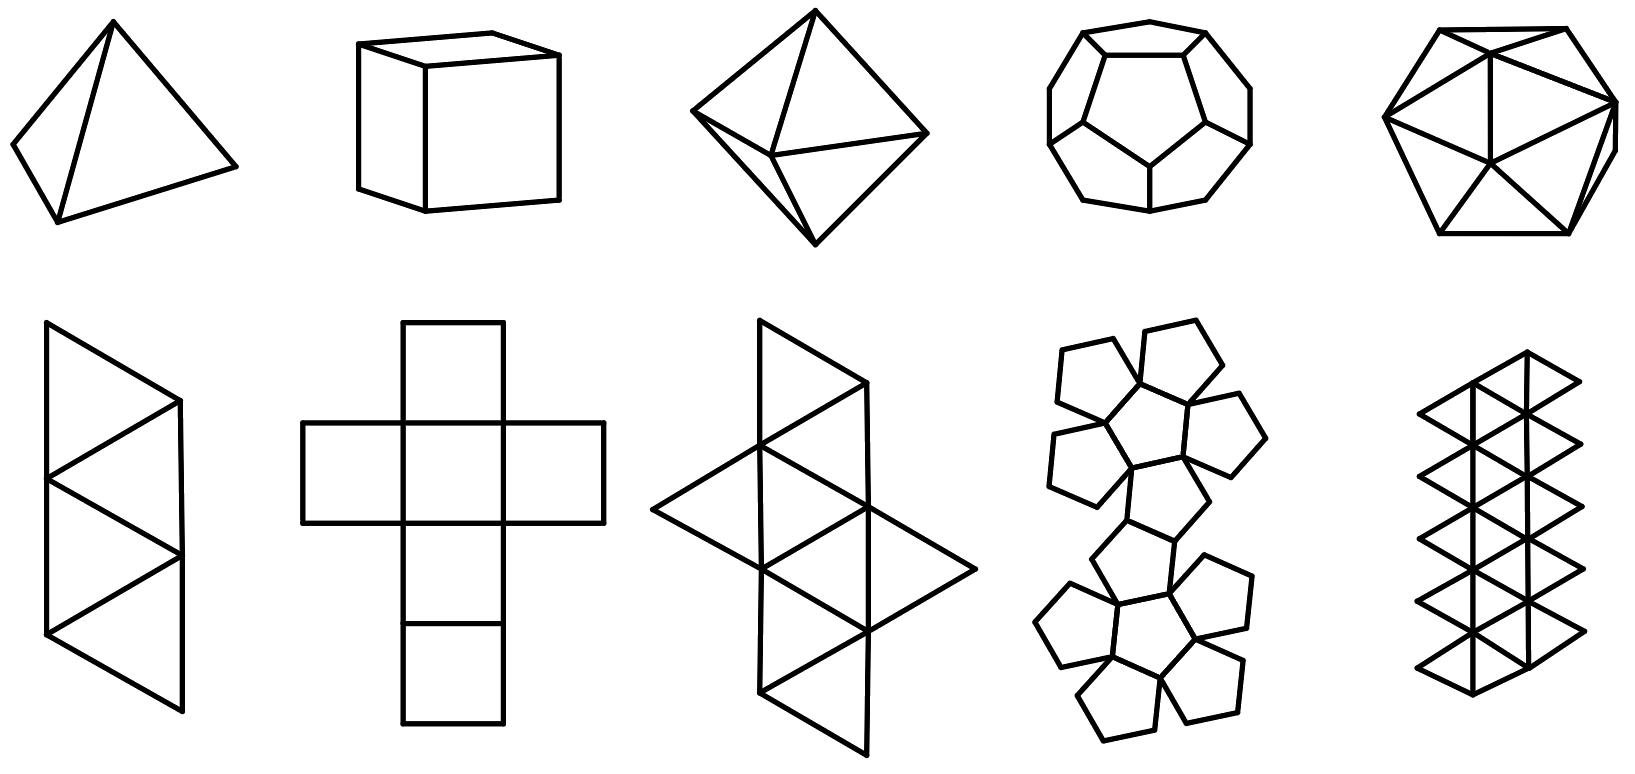
\includegraphics[width=0.9\textwidth]{image/5Platonic1.png}
	\caption{The platonic solids. From left to right with models and unfolding models: the tetrahedron, the cube, the octahedron, the dodecahedron, and the icosahedron}
	\label{fig:platonicSolids}
\end{figure}
%
% 
%
%
%
\noindent \uline{Geometrical parameters}: 
The number of faces, edges, and vertices of each type of platonic solids is described in the Table \ref{tab:tb1}. 
In mathematics, the Euler's formula shows the relationship between total number of vertices ($V$), edges ($E$), and faces ($F$) by the Eq. \ref{equa:eq1}
%
\begin{equation} 
\label{equa:eq1}
\begin{split}
V-E+F=2
\end{split}
\end{equation}
% 
The icosahedron has the largest number of faces with $20$ while the tetrahedron has only $4$ faces. 
If each face of platonic solids has $i$ sides and $k$ edges of the polyhedron meet at each vertex.
The conditions are $i,k$ greater than $3$ ($i,k\geq3$) because every face have at least three edges and at least three edges of faces meet at each vertex.
The faces are equilateral triangle if $i=3$ and changing the values of $k$ will yield the other three types of polyhedron, including the tetrahedron ($k=3$), the octahedron ($k=4$),and the icosahedron ($k=5$). When $i=4$, the faces are square and the cube has $k=3$ edges which meet at each vertex. The last case with $i=4$ of regular pentagons and only $k=3$ will generate the dodecahedron. \\

% %Check p.61 Euler's gem book
%
\begin{table}[H]
\centering
\caption{Properties of polyhedron}
\label{tab:tb1}
\begin{tabular}{|l|c|c|c|c|c|}
\hline
             & Faces & Edges & Vertices & Edges on each face & Edges meeting at each vertex \\ \hline
Tetrahedron  & 4     & 6     & 4        & 3                  & 3                            \\ \hline
Cube         & 6     & 12    & 8        & 4                  & 3                            \\ \hline
Octahedron   & 8     & 12    & 6        & 3                  & 4                            \\ \hline
Dodecahedron & 12    & 30    & 20       & 5                  & 3                            \\ \hline
Icosahedron  & 20    & 30    & 12       & 3                  & 5                            \\ \hline
\end{tabular}
\end{table}
% generate the table from https://www.tablesgenerator.com/#
%
% %Check p.61 Euler's gem book

\noindent The path planning for platonic solids focuses on the rolling of the models through edge-contact. Each edge is shared by two faces and each face may has $e$ edges. Assume that $\Delta $ is the quantity faces which contact at an edge or $E=\frac{1}{2}\Delta $. However, each vertex will be shared by $f$ faces. Then, $V=\frac{\Delta}{f}$. After substituting these two quantities into the Eq. \ref{equa:eq1}, the result is:
%
%
\begin{equation} 
\label{equa:eq2}
\begin{split}
V-E+F &= 2\\
\frac{\Delta}{f} - \frac{1}{2}\Delta + F &= 2\\
\rightarrow F &= \frac{4f}{2e-fe+2f}\\
\end{split}
\end{equation}
%

\noindent From the Eq. \ref{equa:eq2}, the condition is that $2e-fe+2f$ should positive because $F$ and $4f$ are both positive. 
As above requirements with ($e\geq3$) and ($f\geq3$), there are only five pairs of integers ($e,f$) satisfy this condition. 
So, the results of these pairs are shown in the last two columns in Figure \ref{tab:tb1}.\\

\noindent In order to execute the transformation stage, a rotation angle needs to determine in the path planning algorithm.
In the context of regular convex polyhedra, a rotation angle is supplementary with a dihedral angle which is the angle between two connected faces along an edge inside the polyhedra.
The Table \ref{tab:tb2} shows the radii of each solid with the inradius ($r_i$), the midradius ($\rho$), the circumradius ($R$) and the dihedral angles ($\beta$).\\

\begin{table}[h]
\centering
\caption{Geometrical parameters of platonic solids}
\label{tab:tb2}
\begin{tabular}{|l|c|c|c|c|}
\hline
             & $r_d$	                             & $\rho$                    & R	     					      & dihedral angles ($\beta$)	\\ \hline
Tetrahedron  & $\frac{1}{12}\sqrt{6}$    			 & $\frac{1}{4}\sqrt{2}$     & $\frac{1}{4}\sqrt{6}$              & $\cos^{-1}(\frac{1}{3})$                       \\ \hline
Cube         & $\frac{1}{2}$                         & $\frac{1}{2}\sqrt{2}$     & $\frac{1}{2}\sqrt{3}$              & $\frac{1}{2}\pi$                \\ \hline
Octahedron   & $\frac{1}{6}\sqrt{6}$    			 & $\frac{1}{2}$    	     & $\frac{1}{2}\sqrt{2}$      		  & $\cos^{-1}(-\frac{1}{3})$               \\ \hline
Dodecahedron & $\frac{1}{20}\sqrt{250+110\sqrt{5}}$  & $\frac{1}{4}(3+\sqrt{5})$ & $\frac{1}{4}(\sqrt{15}+\sqrt{3})$  & $\cos^{-1}(-\frac{1}{5}\sqrt{5})$              \\ \hline
Icosahedron  & $\frac{1}{12}(3\sqrt{3}+\sqrt{15})$   & $\frac{1}{4}(1+\sqrt{5})$  & $\frac{1}{4}\sqrt{10+2\sqrt{5}}$  & $\cos^{-1}(-\frac{1}{3}\sqrt{5})$               \\ \hline
\end{tabular}
\end{table}

\clearpage
\newpage
%\vspace{1in}
%\begin{table}%[h!]
%	\centering
%	\caption{Optimized Parameter Values}
%	\begin{tabular}{llllp{7em}p{7em}l}
%		\toprule
%		Type of Controller & Parameter    & Xmax & Xmin & \raggedright Iter. reqd. for convergence & Optimized value & $W_\mathrm{min}$ \\ \midrule
%			PSO-SOSMC        & $c_1$        & 5    & 0.1  & 37                                       & 4.75            & 68.43 \\
%			                 & $c_2$        & 5    & 0.1  & 10                                       & 4.273           & 20.45 \\
%			                 & $\lambda_1 $ & 5    & 0.1  & 37                                       & 2.75            & 68.43\\
%			                 & $\lambda_2 $ & 5    & 0.1  & 10                                       & 3.59            & 20.45\\
%			                 & $W_1 $       & 1    & 0.05 & 37                                       & 0.43            & 68.45\\
%			                 & $W_2 $       & 1    & 0.05 & 10                                       & 0.218           & 20.43\\ \cmidrule(lr){2-7}
%			PSO-BELBIC       & $W_1$        & 5    & 0.1  & 36                                       & 4.5             & 27.34 \\
%			                 & $W_2$        & 5    & 0.1  & 14                                       & 4.5             & 61.63 \\
%			                 & $G_1$        & 5    & 0.1  & 36                                       & 1.4             & 27.34 \\
%			                 & $G_2$        & 5    & 0.1  & 14                                       & 1.4             & 61.63\\ \bottomrule
%		\end{tabular}
%\end{table}
\section{ALGORITHM\textbackslash METHODOLOGY}
\label{sec:Algorithm}
\subsection{Path Planning Based Rolling Contact}
\noindent\uline{Rolling on discretized surfaces}:
The surface contacts between platonic solids and the plane can be categorized into three types as shown in Figure \ref{fig:gridPlatonic} including square shape for cube, triangle shape for tetrahedron, octahedron, and dodecahedron, pentagon shape for dodecahedron. 
The bottom surface of a cube occupies each square on the grid when the path planning process is executed. This property is applied for triangular grid with different rotation angle. 
In physics, the rotation angle of the cube is $\pi/2(rad)$ while the rotation angles of tetrahedron, octahedron, icosahedron and dodecahedron are $\pi-\arctan{(2\sqrt{2})}$, $\pi-2\arctan{\sqrt{2}}$, $\arccos{(-\sqrt{5}/3)}$, and $\pi-\arccos{(-\sqrt{5}/5)}$ in radian respectively.\\

\noindent{The square grid has $\pi/2$ at all corners while the triangular grid has $\pi/3$ between two arbitrary edges at a vertex. 
In the case of dodecahedron rolling contact, the Figure \ref{fig:gridPlatonic}d shows the two types of connections between pentagons where the first case has a gap (Figure \ref{fig:gridPlatonic}c) and the other has overlap pentagon connection. 
A regular pentagon has five interior angles of $\ang{108}$ which generate a gap between three pentagons surrounding because of $3*\ang{108}=\ang{324}$, which is different $\ang{360}$ of the full circle.
Another case of four overlap pentagons with $4*\ang{108}=\ang{432}$ is greater than the circle of $\ang{360}$. 
The path planning through rolling of the dodecahedron solid can be categorized into two these cases. 
It would be found the possible paths in the first case of dodecahedron without overlap rolling while the second case with overlap rolling cannot guarantee the paths.}

%
\begin{figure}[h]
\centering
	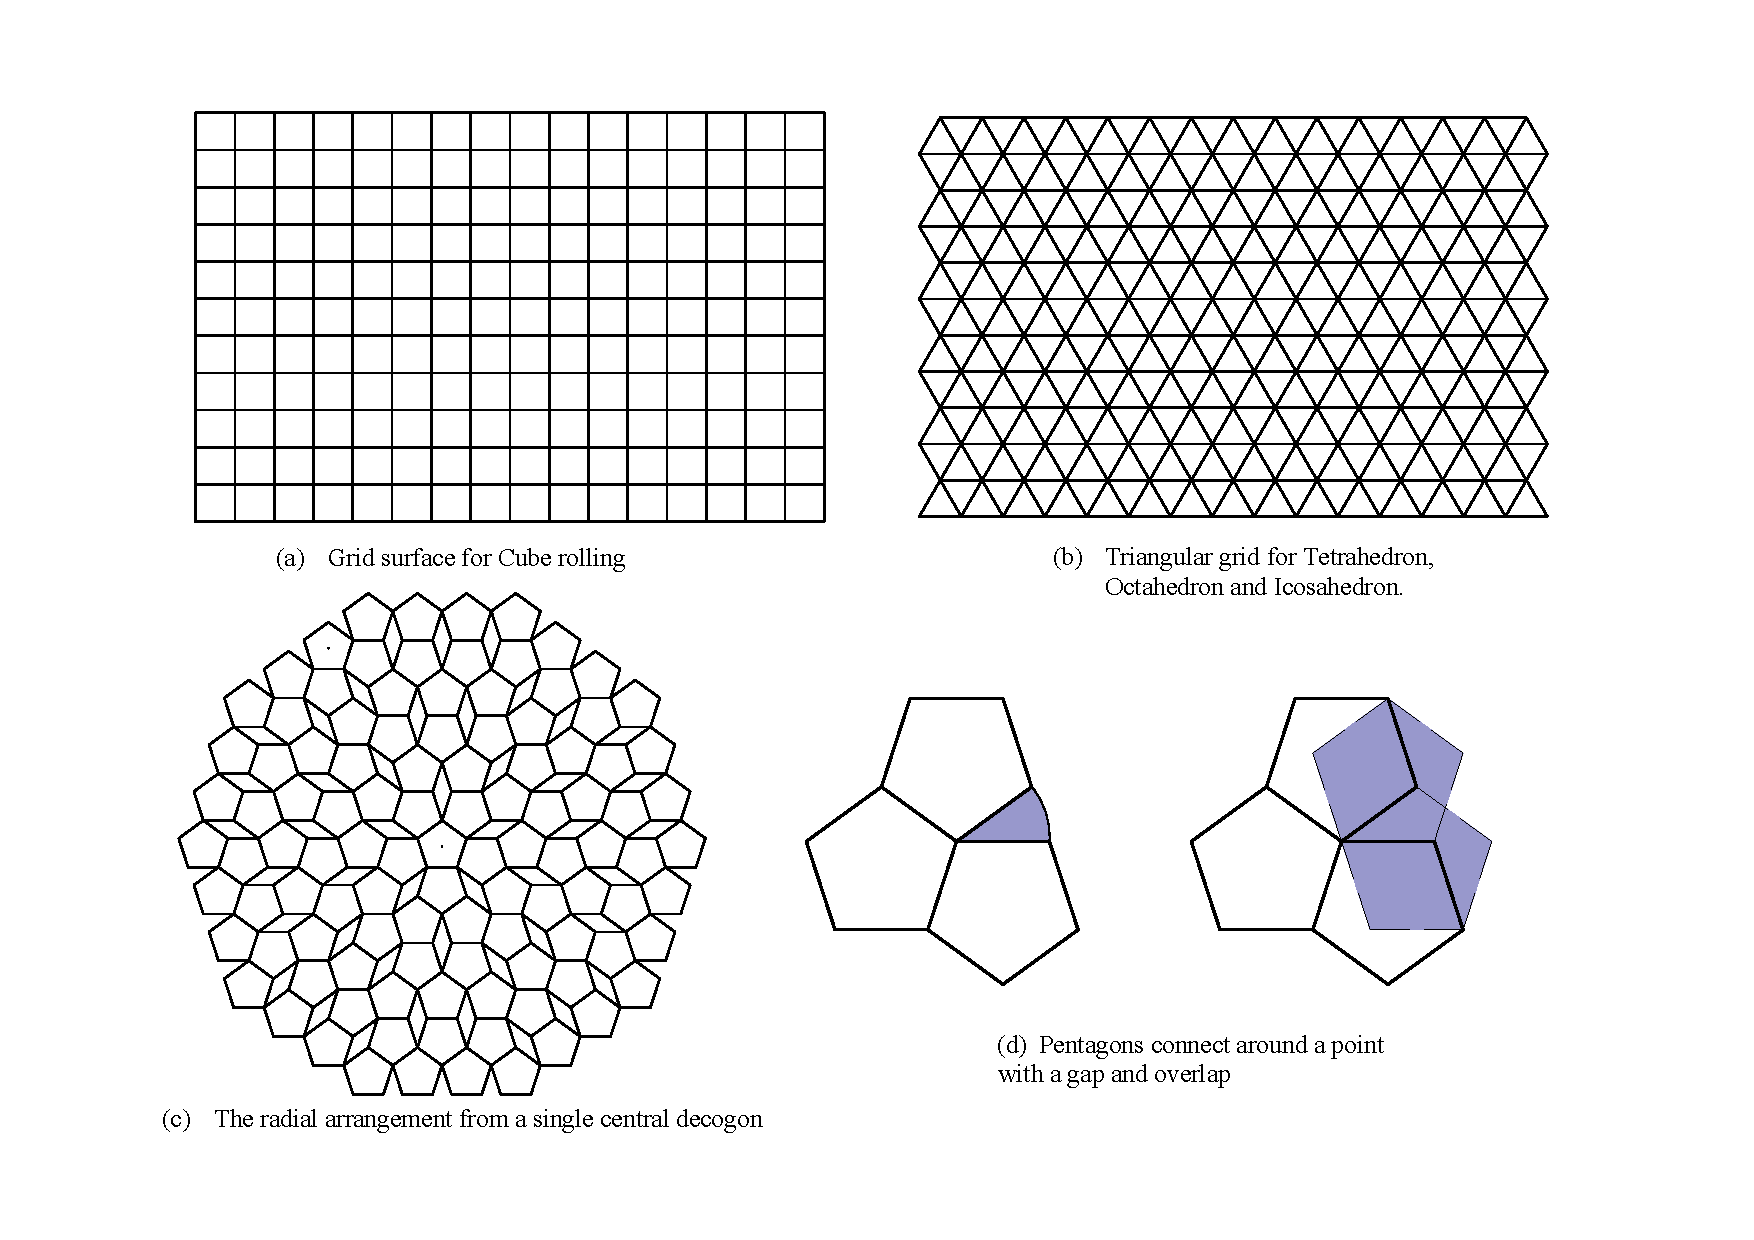
\includegraphics[width=1\textwidth]{image/gridPlatonic.pdf}
	\caption{Grid of platonic solids}
	\label{fig:gridPlatonic}
\end{figure}


\noindent\uline{Rodrigues' roatation}: It is assumed that the motion of rolling the platonic solids is a pure rolling without slipping or spinning at the line contact.
Rolling the platonic solids means rolling all its vertices in $3D$ environment indicated by changing the coordinates. There were several algorithms to transform vertices stored in a matrix in $3D$ space. In this case, the Rodrigues's rotation method in \cite{Dai_Rodrigues_2015} is used to represent the rotation matrix in the path planning algorithm. The method is explained in the Section \ref{sec:eva}. 
\textcolor{red}{Check the paper "Kinematics of Spherical Robots Rolling Over 3D Terrains"}.

%
\clearpage
\newpage
\noindent\uline{Algorithms}:
Due to the different surface contacts, there are three types of direction for the rolling of platonic solids. As shown in the Figure \ref{fig:rollingDir}, the cube has four directions with the square surface contact while tetrahedron, octahedron and icosahedron have three rolling directions with the triangular surface contact. The dodecahedron with pentagon surface contact has five rolling directions. In the case of rolling cube, the surface contact is surrounded by four edges which means there are four possible directions through the edges. In this work, the proposed path planning algorithm deals with rolling from initial configuration within the position and orientation to the goal within the same position but different orientation. While rolling on the smooth plane, the platonic solid models will contact to the plane though their edges.\\

\noindent The Algorithm \ref{alg:rollingPath} shows that path planning for cube rolling based on tree graph search has some important steps. The first step is to initial the coordinates and the orientations of the initial cube and the target cube which is stored as the initial path. The same as tree expansion, cube will roll in four different directions including the right, left, up and down is the next step. From these new positions and orientations, the cubes will continue expand with only three directions to avoid return the previous positions. An example for this step is that from the initial coordinate the cube achieves a new position after doing rolling for right direction, the new three positions of the cube by rolling through right, up, and down direction. After implementing the expansion steps through rolling, the function of checking whether updated models reach the goal is called through the loop. By that means, the loop will stop when reaching the goal whereas the loop will continue to execute and store new models to the initial path. While the searching algorithm is executing, the data structure is used to store the positions and orientations from the start to the current. This process runs in time $O(|E|^3)$ (where $|E|$ is the number of updated cubes) which causes the longer the running time of the searching technique. \\

\noindent  
% 
%
%
%%==================================================================================
\begin{figure}[h]
\centering
	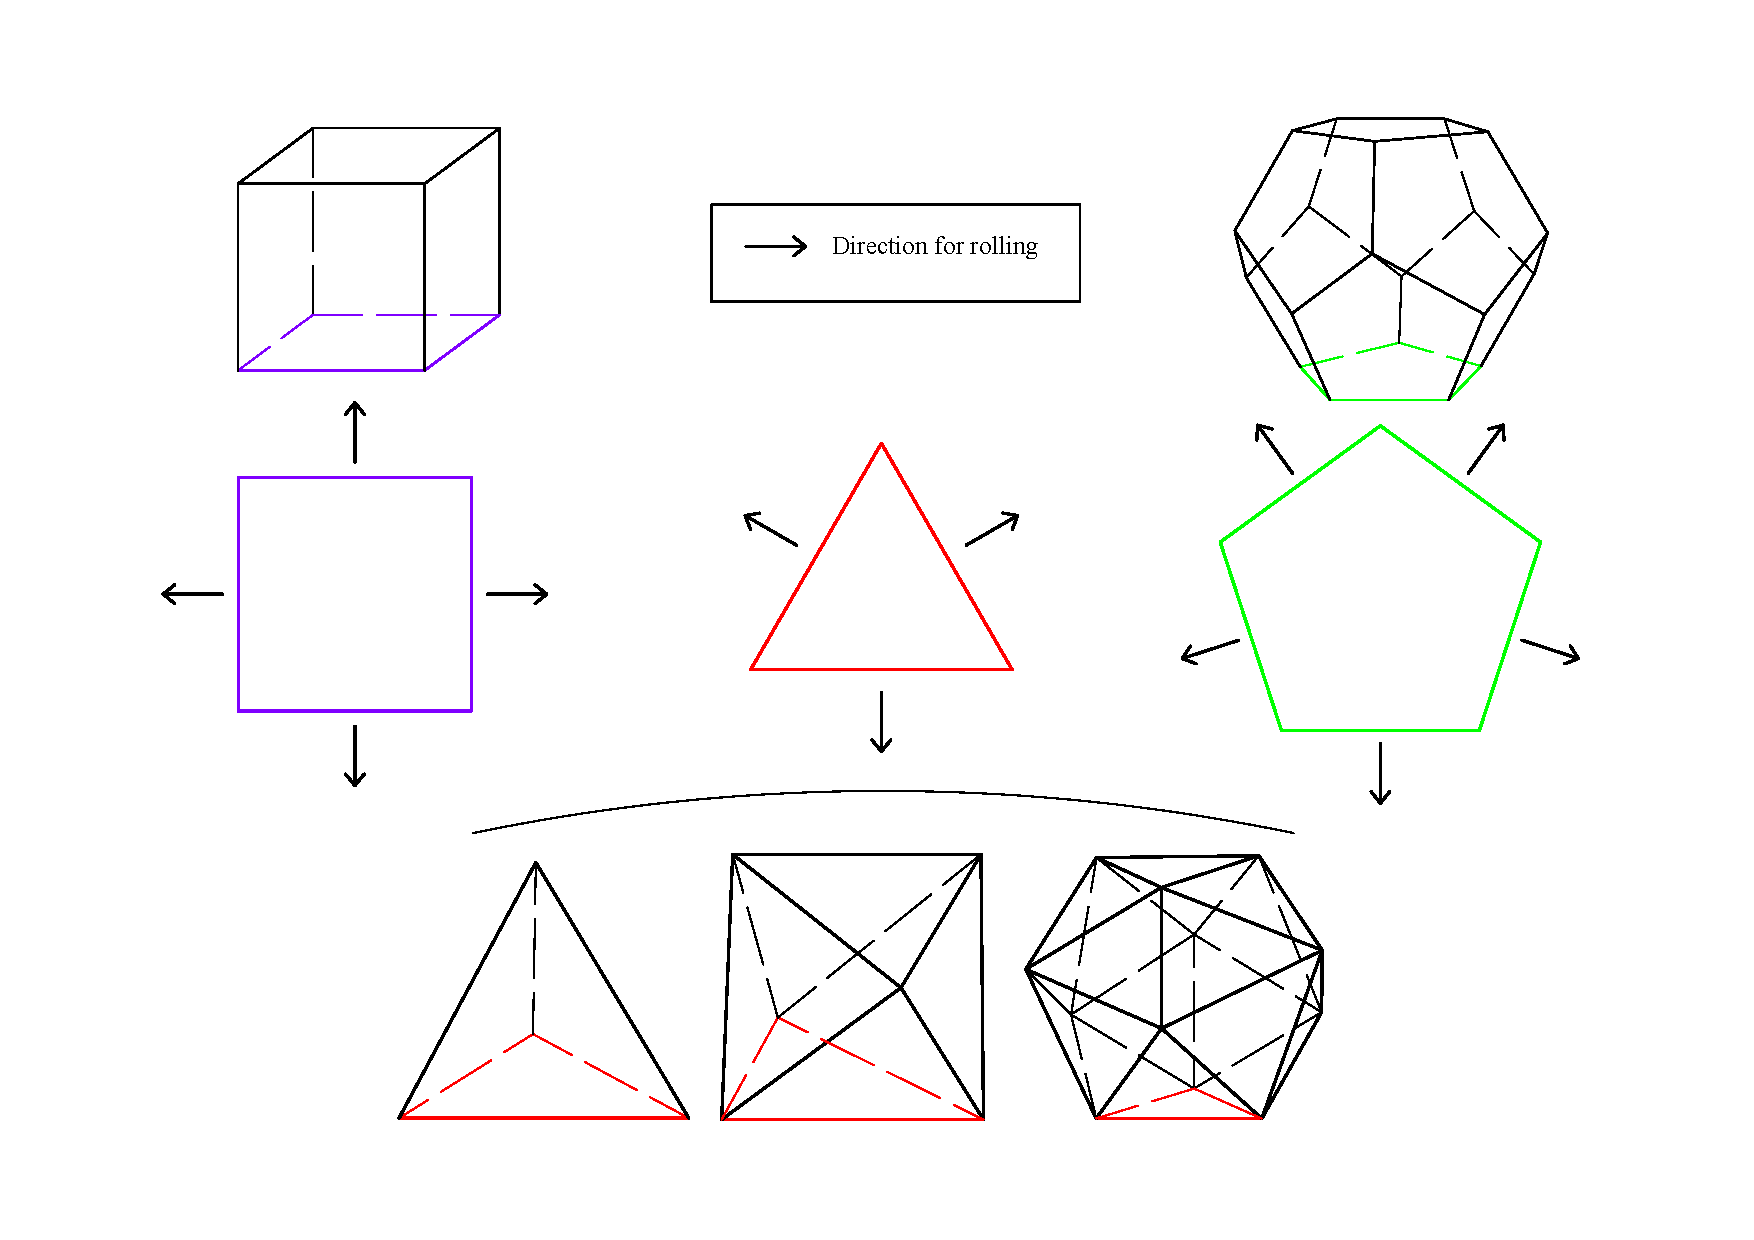
\includegraphics[width=1\textwidth]{image/rollingDir2.pdf}
	\caption{Rolling direction for each types of platonic solids}
	\label{fig:rollingDir}
\end{figure}
%
% 
%
%
%%==================================================================================
%
%
%%==================================================================================
\clearpage
\newpage
\begin{algorithm}
\caption{Path planning based rolling contact for Cube model.\label{alg:rollingPath}}
\begin{algorithmic}[1]
\Procedure {CubePathPlanning}{$S_p$, $G_p$}               \Comment{Find the shortest path from start to goal position with different orientation}
	\State $flag$ $\leftarrow$ $false$
	\State $Path[S_p]$ $\leftarrow$ $S_p$
	\State $newPoints$ $\leftarrow$ \textsc{rolling4Directions}($S_p$)	\Comment{Generate first four updated points}
	\While{$newPoints$ $!=$ $G_p$} 
		\State $updatedPoints$ $\leftarrow$ \textsc{treeExploration}($newPoints$)	\Comment{Update new three right rolling models}
		\State $n$ $\leftarrow$ \textit{size}$(updatedPoints)$
		\For{$i\gets 0, n$}		
			\For{$j\gets 1, n$}	
				\If {$updatedPoints[i]$ $=$ $updatedPoints[j]$}
					\State \textit{remove}($updatedPoints[i]$)
				\EndIf
			\EndFor
		\EndFor		
		\State $flag$ $\leftarrow$ \textsc{checkingTargetPoint}($updatedPoints$) 	\Comment{Compare updated points with goal point}  	
			\If {$flag$ $=$ $true$}
				\State \Return {$Path[S_p,G_p]$} 								    \Comment{Store new point to $Path$}
			\EndIf
			\State $newPoints$ $=$ $updatedPoints$ 
	\EndWhile
	\State  \Return {\textit{"no path found"}} 	
\EndProcedure
%\Statex
\Procedure {rolling4Directions}{$S_p$}\Comment{Generate new points in different direction of rolling}
	\State $(newRightPoint,newLeftPoint,newUpPoint,newDownPoint)$ $\leftarrow$ \textsc{rollingContact}($S_p$)				
	\State \Return{$newPoints$ $\leftarrow$ $(newRightPoint,newLeftPoint,newUpPoint,newDownPoint)$}
\EndProcedure
%%\Statex
\Procedure {treeExploration}{$newPoints$}
	\If {$dir$ $=$ $right$}
		\State  $updatedPoints$ $\leftarrow$  $(newRightPoint,newUpPoint,newDownPoint)$
	\ElsIf {$dir$ $=$ $left$}
		\State $updatedPoints$ $\leftarrow$  $(newLeftPoint,newUpPoint,newDownPoint)$
	\ElsIf {$dir$ $=$ $up$}
		\State $updatedPoints$ $\leftarrow$  $(newRightPoint,newLeftPoint,newUpPoint)$
	\Else %{$dir$ $=$ $right$}
		\State $updatedPoints$ $\leftarrow$  $(newRightPoint,newLeftPoint,newDownPoint)$
	\EndIf
	\State \Return {$updatedPoints$}
\EndProcedure
%\Statex
\Procedure {checkingTargetPoints}{$updatedPoints$,$G_p$}
	\If {$updatedPoints$ $=$ $G_p$}									\Comment{Consider both position and orientation}
		\State $flag$ $\leftarrow$ $true$
	\EndIf
	\State \Return {$flag$}
\EndProcedure
\end{algorithmic}
\end{algorithm}


%\clearpage
\newpage
%----------------------------------
\subsection{Tree Exploration Algorithm}
The node tree exploration for searching algorithm described in Algorithm \ref{alg:rollingPath} is similar to non-recursive depth-first-search algorithm. The graph search in the Figure \ref{fig:nodeTree} shows the expansion from the $root$ with node $S$ to multi-level from $1^{st} level ... n^{th} level$ for the case study of a cube solid.
%
Each nodes indicates the position of the cube's center and the orientation of the cube. The node $S$ means Start-Point while $R,L,U,D$ are labelled for four different directions including right, left, up and down respectively. 
%
For each iterations, a tree with a node including $3D$ coordinate and orientation is stored in each levels. At the same time, the algorithm of checking the goal configuration will be called to check whether the current executing level achieves the target.\\


\noindent In other cases of tetrahedron, octahedron and icosahedron with the triangular grid (Figure \ref{fig:gridPlatonic}b), there are three directions at the first rolling and only two directions for the rest of path-finding process.
%
Only the case of dodecahedron has the different approach from the algorithm. The path planning algorithm depends on the environment including gaps or overlaps between two pentagon connections as can be seen in the Figure \ref{fig:gridPlatonic}b.
%
\vskip 0.5cm
\begin{figure}[h]
	This is the node tree for searching algorithm. Different colors indicate different level of searching steps. %\vskip 0.5cm


\tikzset{
	level/.style={sibling distance=35mm/#1},
	treenode/.style={align=center,inner sep=0pt},
	% Black nodes
	node_black/.style={treenode,circle,black,draw=black,very thick,text width=0.5cm},
	% Red nodes
	node_red/.style={treenode,circle,red,draw=red,very thick,text width=0.5cm},
	% Blue nodes
	node_blue/.style={treenode,circle,blue,draw=blue,very thick,text width=0.5cm},
	% Nil nodes
	node_nil/.style={treenode,rectangle,fill=black,minimum width=0.3cm,minimum height=0.3cm}
}
\begin{tikzpicture}
\node[node_red] (z){$S$}
  child {node[node_black] (a) {$R$}								%%% Right
    child[black] {node[node_black]  (b) {$R$}
      child {node (b1) {$\vdots$}
       child {node[node_black] (b11) {$R$}}
      }
      child {node (b2) {$\vdots$}
       child {node[node_black] (b12) {$U$}}
      }
    }
    child[black] {node[node_black] (g) {$D$}
      child {node (g1) {$\vdots$}
       child {node[node_black] (g11) {$R$}}
      }
      child {node (g2) {$\vdots$}
       child {node[node_black] (g12) {$U$}}
      }
    }
  }
   child[red] {node[node_red] (d) {$L$}                    %%%% LEft - the shortest parth
      child[black] {node[node_black]  (e) {$L$}
        child {node (e1) {$\vdots$}
         child {node[node_black] (e11) {$R$}}
        }
        child {node (e2) {$\vdots$}
         child {node[node_black] (e12) {$L$}}
        }
      }
      child[red] {node[node_red] (f) {$D$}
        child[black] {node (f1) {$\vdots$}
         child[black] {node[node_black] (f11) {$U$}}
        }
        child[red] {node (f2) {$\vdots$}
         child[red] {node[node_red] (f12) {$D$}}
        }
      }
    }
    child[black] {node[node_black] (m) {$U$}      %%% Up
      child {node[node_black]  (n) {$U$}
        child {node (n1) {$\vdots$}
         child {node[node_black] (n11) {$R$}}
        }
        child {node (n2) {$\vdots$}
         child {node[node_black] (n12) {$L$}}
        }
      }
      child {node[node_black] (o) {$L$}
        child {node (o1) {$\vdots$}
         child {node[node_black] (o11) {$U$}}
        }
        child {node (o2) {$\vdots$}
         child[blue] {node[node_blue] (o12) {$R$}}
        }
      }
    }
  child[black] {node[node_black]  (j) {$D$}   %%% Down
    child {node[node_black] (k) {$D$}
      child {node {$\vdots$}
       child[blue] {node[node_blue] (k11) {$R$}}
      }
      child {node {$\vdots$}
       child {node[node_black] (k12) {$D$}}
      }
    }
    child {node[node_black] (l) {$L$}
    child {node {$\vdots$}
     child {node[node_black] (l11) {$U$}}
    }
    child {node (c){$\vdots$}
     child {node[node_black] (l12) {$L$}
            child [grow=right] {node (r) {$level^n$} edge from parent[draw=none]
              child [grow=up] {node (s) {$\vdots$} edge from parent[draw=none]
                child [grow=up] {node (t) {$level^2$} edge from parent[draw=none]
                  child [grow=up] {node (u) {$level^1$} edge from parent[draw=none]
                   child [grow=up] {node (u) {$root$} edge from parent[draw=none]}
                                   }
                                 }
                               }
                               }
            }
          }
         }
};
\path (b) -- (g) node [midway] {$\cdots$};\path (n) -- (o) node [midway] {$\cdots$};
\path (e) -- (f) node [midway] {$\cdots$};
\path (k) -- (l) node [midway] {$\cdots$};
\path (b11) -- (b12) node [midway] {$\cdots$};
\path (g11) -- (g12) node [midway] {$\cdots$};\path (n11) -- (n12) node [midway] {$\cdots$};
\path (e11) -- (e12) node [midway] {$\cdots$};\path (o11) -- (o12) node [midway] {$\cdots$};
\path (f11) -- (f12) node [midway] {$\cdots$};
\path (k11) -- (k12) node [midway] {$\cdots$};
\path (l11) -- (l12) node [midway] {$\cdots$};
\end{tikzpicture}

%% take notes


\begin{tikzpicture}
%\node[node_black] (n12) {}
%\node[node_red] (n12) {}
%\node[node_blue] (n12) {}
\end{tikzpicture}


	\caption{Tree Exploration of Cube Rolling}
\label{fig:nodeTree}
\end{figure}

\noindent Starting form the root $S$, path planning based rolling of the cube model at the first level of expansion will generate to four different direction $R,L,U,D$. In the next level, the cube can only roll with three directions without rolling back to the previous position.  
An example of the second level is that node $R$ will roll to right, up, and down directions indicated by node $R,U,D$ respectively.\\
% 

\noindent To eliminate the processing time in the proposed algorithms, whenever any updated points achieved the same position and orientation, these nodes will merge at that $level$. An example from Figure \ref{fig:nodeTree} shows two updated nodes $R$ (blue node) at $(n-1)^{th} level$ have achieved the same position. The next path is generated from this merged nodes. 
%
From the tree exploration algorithm, the result can show only one path or various paths which depends on the initial and goal configuration. The first path is the shortest path because the executing time is shortest based on the condition of achieving goal configuration.
% 
%\vskip 0.5cm
%\begin{figure}[h]
%    \centering
%	\tikzset{
	level/.style={sibling distance=35mm/#1},
	treenode/.style={align=center,inner sep=0pt},
	% Black nodes
	node_black/.style={treenode,circle,black,draw=black,very thick,text width=0.4cm},
	% Red nodes
	node_red/.style={treenode,circle,red,draw=red,very thick,text width=0.4cm},
	% Blue nodes
	node_blue/.style={treenode,circle,blue,draw=blue,very thick,text width=0.4cm},
	% Nil nodes
	node_nil/.style={treenode,rectangle,fill=black,minimum width=0.3cm,minimum height=0.3cm}
}
\begin{tikzpicture}

\node[node_red] (z){$S$}
  child {node[node_black] (a) {$R$}								%%% Right
    child[black] {node[node_black]  (b) {$R$}
      child {node (b1) {$\vdots$}
       child {node[node_black] (b11) {$R$}}
      }
      child {node (b2) {$\vdots$}
       child {node[node_black] (b12) {$U$}}
      }
    }
    child[black] {node[node_black] (g) {$D$}
      child {node (g1) {$\vdots$}
       child {node[node_black] (g11) {$R$}}
      }
      child {node (g2) {$\vdots$}
       child {node[node_black] (g12) {$U$}}
      }
    }
  }
   child[red] {node[node_red] (d) {$L$}         %% LEft - the shortest parth
      child[black] {node[node_black]  (e) {$L$}
        child {node (e1) {$\vdots$}
         child {node[node_black] (e11) {$R$}}
        }
        child {node (e2) {$\vdots$}
         child {node[node_black] (e12) {$L$}}
        }
      }
      child[red] {node[node_red] (f) {$D$}
        child[black] {node (f1) {$\vdots$}
         child[black] {node[node_black] (f11) {$U$}}
        }
        child[red] {node (f2) {$\vdots$}
         child[red] {node[node_red] (f12) {$L$} 
         	child[black] {node[node_black] (g44) {$L$}}
         	child[red] {node[node_red] (g22) {$G$}} 
         	child[black] {node[node_black] (g33) {$D$}}  
          }
        }
      }
    }
    child[black] {node[node_black] (m) {$U$}      %%% Up
      child {node[node_black]  (n) {$U$}
        child {node (n1) {$\vdots$}
         child {node[node_black] (n11) {$R$}}
        }
        child {node (n2) {$\vdots$}
         child {node[node_black] (n12) {$L$}}
        }
      }
      child {node[node_black] (o) {$L$}
        child {node (o1) {$\vdots$}
         child {node[node_black] (o11) {$U$}}
        }
        child {node (o2) {$\vdots$}
         	child[blue] {node[node_blue] (o12) {$R$}
         		child[black] {node[node_black] (merge1) {$R$}  }
         		child[black] {node[node_black] (merge2) {$U$}  }
         		child[black] {node[node_black] (merge3) {$D$}  }
                  }
              }
           }
    }
  child[black] {node[node_black]  (j) {$D$}   %%% Down
    child {node[node_black] (k) {$D$}
      child {node {$\vdots$}
       child[blue] {node[node_blue] (k11) {$R$}}
      }
      child {node {$\vdots$}
       child {node[node_black] (k12) {$D$}}
      }
    }
    child {node[node_black] (l) {$L$}
    child {node {$\vdots$}
     child {node[node_black] (l11) {$U$}}
    }
    child {node (c){$\vdots$}
     child {node[node_black] (l12) {$L$}
%            child [grow=right] {node (r) {$level^n$} edge from parent[draw=none]
%              child [grow=up] {node (s) {$\vdots$} edge from parent[draw=none]
%                child [grow=up] {node (t) {$level^2$} edge from parent[draw=none]
%                  child [grow=up] {node (u) {$level^1$} edge from parent[draw=none]
%                   child [grow=up] {node (u) {$root$} edge from parent[draw=none]}
%                                   }
%                                 }
%                               }
%                               }
            }
          }
         }
};
\path (b) -- (g) node [midway] {$\cdots$};
\path (n) -- (o) node [midway] {$\cdots$};
\path (e) -- (f) node [midway] {$\cdots$};
\path (k) -- (l) node [midway] {$\cdots$};
\path (b11) -- (b12) node [midway] {$\cdots$};
\path (g11) -- (g12) node [midway] {$\cdots$};
%\path (g22) -- (g33) node [midway] {$\cdots$};
\path (n11) -- (n12) node [midway] {$\cdots$};
\path (e11) -- (e12) node [midway] {$\cdots$};
\path (o11) -- (o12) node [midway] {$\cdots$};
\path (f11) -- (f12) node [midway] {$\cdots$};
\path (k11) -- (k12) node [midway] {$\cdots$};
\path (l11) -- (l12) node [midway] {$\cdots$};
\path (g33) -- (merge1) node [midway] {$\cdots$};

%\begin{tikzlegend}[legend entries={monopolist profit within entry allowance,
%      monopolist profit within entry deterrence,something else},
%        legend style={at={(0,-1)},anchor=north west}, legend cell align=left]
%     \addlegendimage{dotted,sharp plot}
%     \addlegendimage{sharp plot}
%     \addlegendimage{dashed, sharp plot}
%\end{tikzlegend}   
   
\end{tikzpicture}
%	\caption{Merge Nodes of Cube Rolling}
%\label{fig:mergeNode}
%\end{figure}
%
%----------------------------------
\clearpage
\newpage
\section{EVALUATION}
\uline{\textbf{Simulations}}: Our algorithm was implemented in MATLAB. Three case studies of path planning are considered for validation: same location and different orientation between initial configuration and goal configuration, long distance between two configuration, and bi-direction path finding.\\

\noindent\uline{\textbf{Cube solid}}:
Writing about cube solid properties\\

\noindent\uline{Case study 1}: Dennis also went his own way and divided the sides of the triangles into equal-angles (as measured from the center of the geodesic), instead of equal-length pieces. This technique is slightly more effective at evenly distributing the triangles across the surface of the sphere. For example, compare an octahedron subdivided with frequency 20, using the linear technique (as outlined by the quiz) versus the angular technique Dennis used in this picture. Note how the linear technique has the triangles piling up along the edges of the original face of the octahedron, where the radial technique does a better job of spacing them out.
\begin{center}
\begin{figure}[h]
\subfigure[The initial configuration is the same position but different orientation with goal configuration]{
	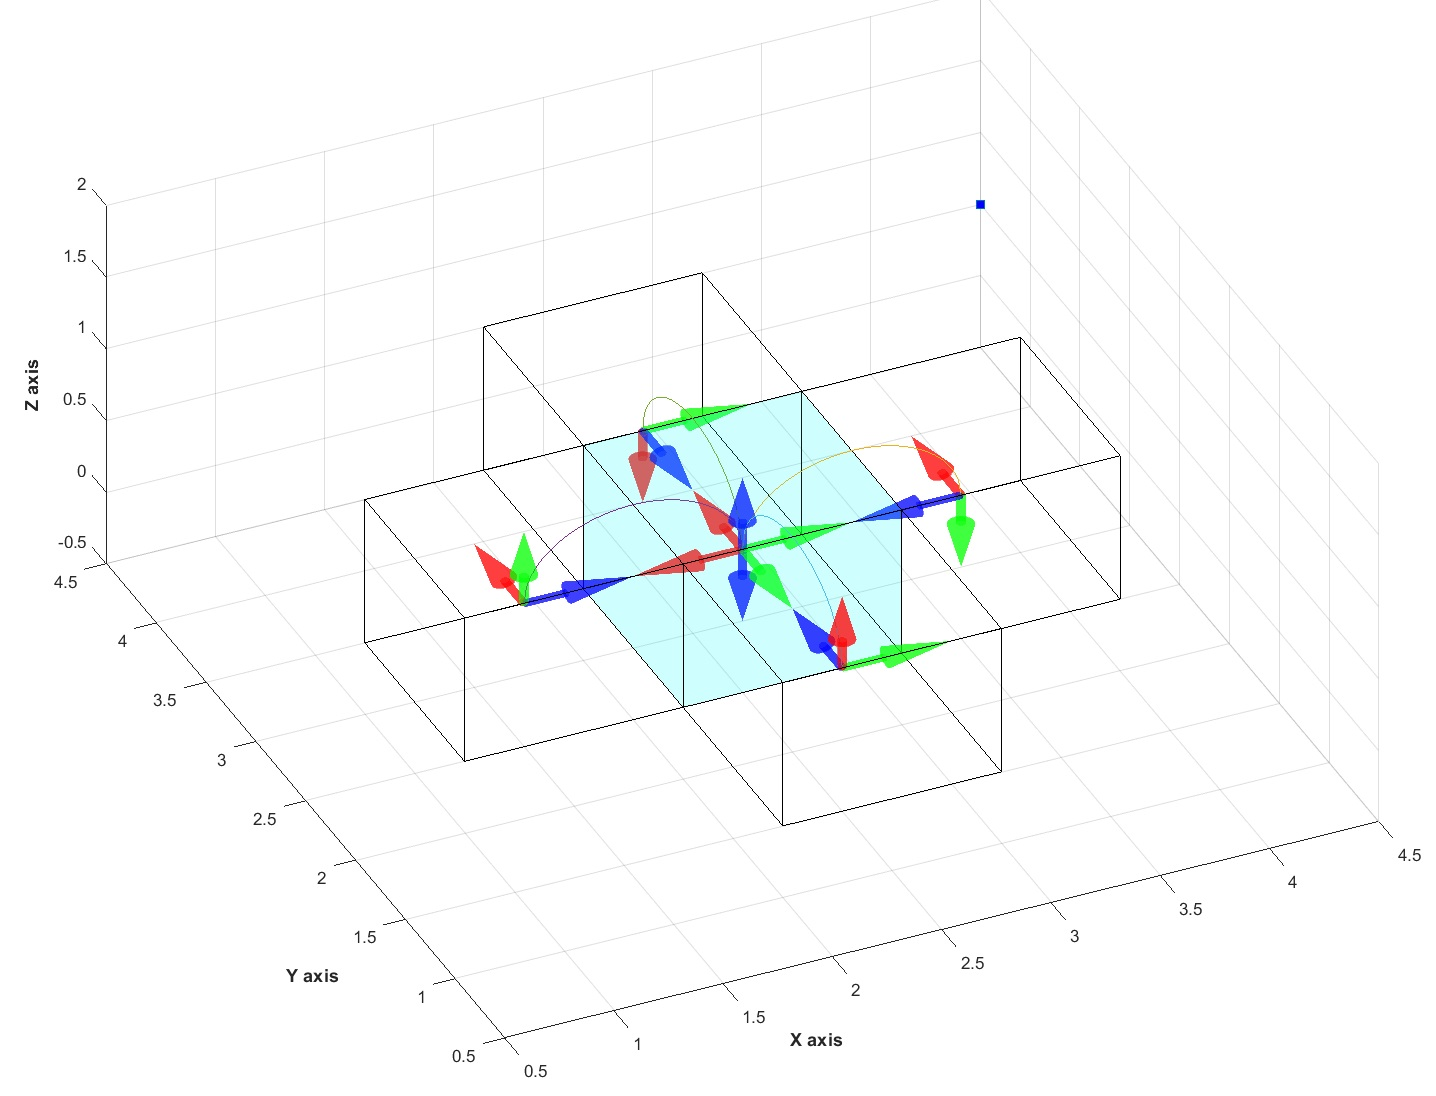
\includegraphics[width=0.5\textwidth]{image/cube11.jpg}
	\label{fig:Cube1Case1}
	}
\hfill
\subfigure[First four paths of the cube rolling]{
	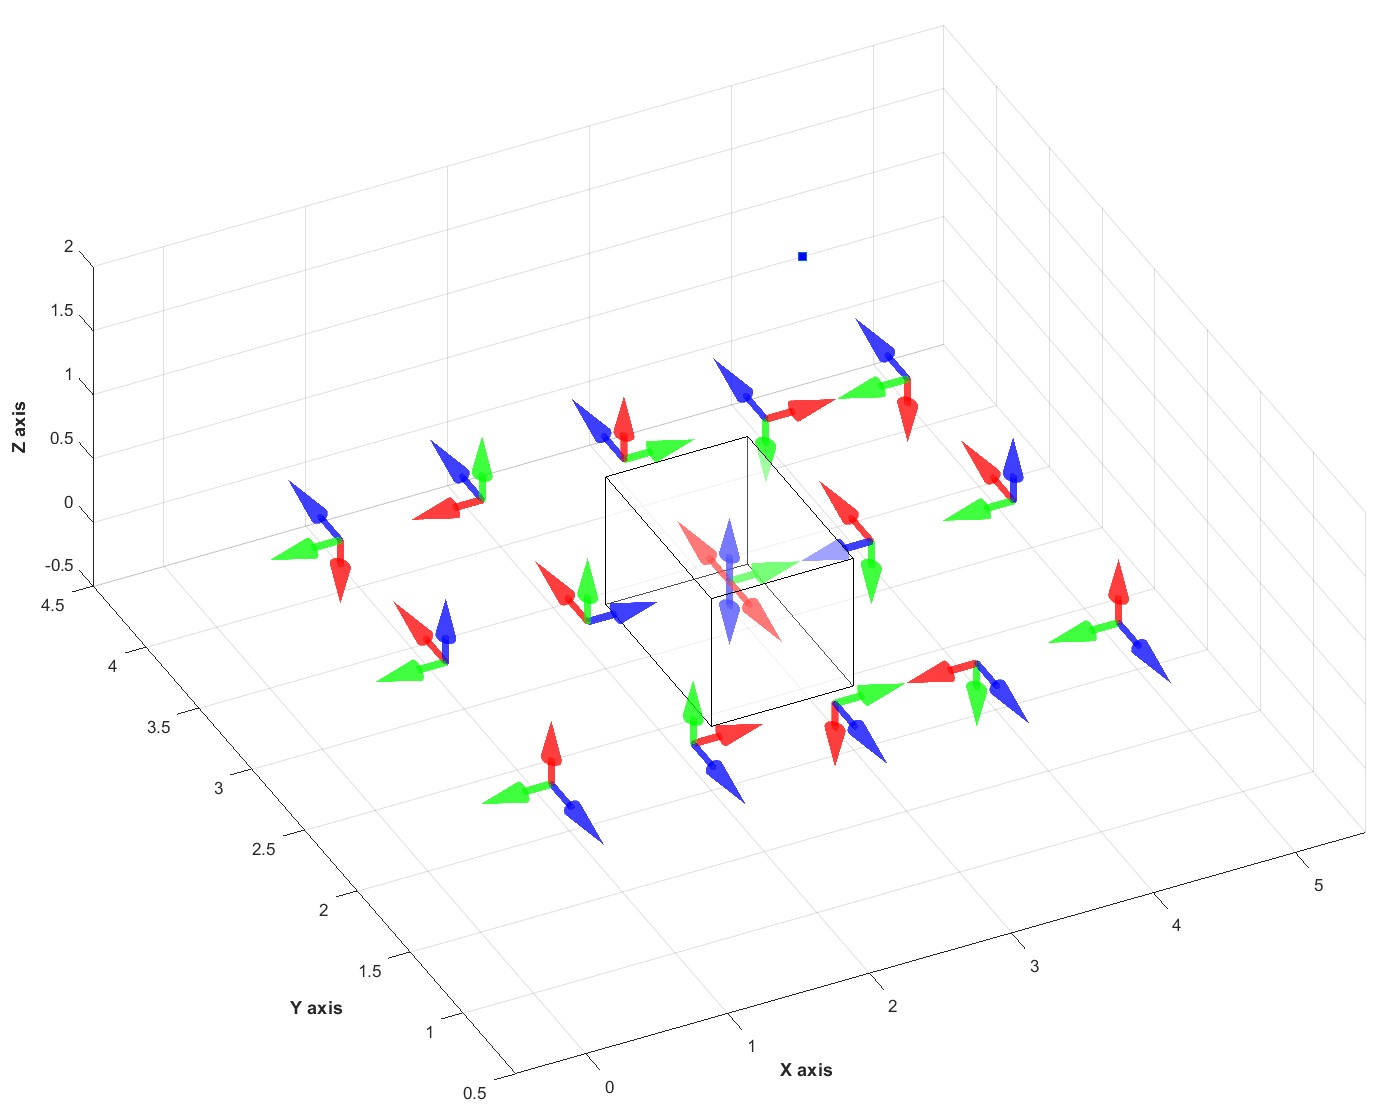
\includegraphics[width=0.5\textwidth]{image/cubePath4Dirs.jpg}
	\label{fig:Cube2Case1}
	}
\caption{Blah Blah}
\end{figure}
\end{center}

\noindent\uline{Case study 2}: Long distance between two configuration:
Dennis also went his own way and divided the sides of the triangles into equal-angles (as measured from the center of the geodesic), instead of equal-length pieces. This technique is slightly more effective at evenly distributing the triangles across the surface of the sphere. For example, compare an octahedron subdivided with frequency 20, using the linear technique (as outlined by the quiz) versus the angular technique Dennis used in this picture. Note how the linear technique has the triangles piling up along the edges of the original face of the octahedron, where the radial technique does a better job of spacing them out.
%\begin{figure}[h]
%	\centering
%		\begin{subfigure}[t]
%			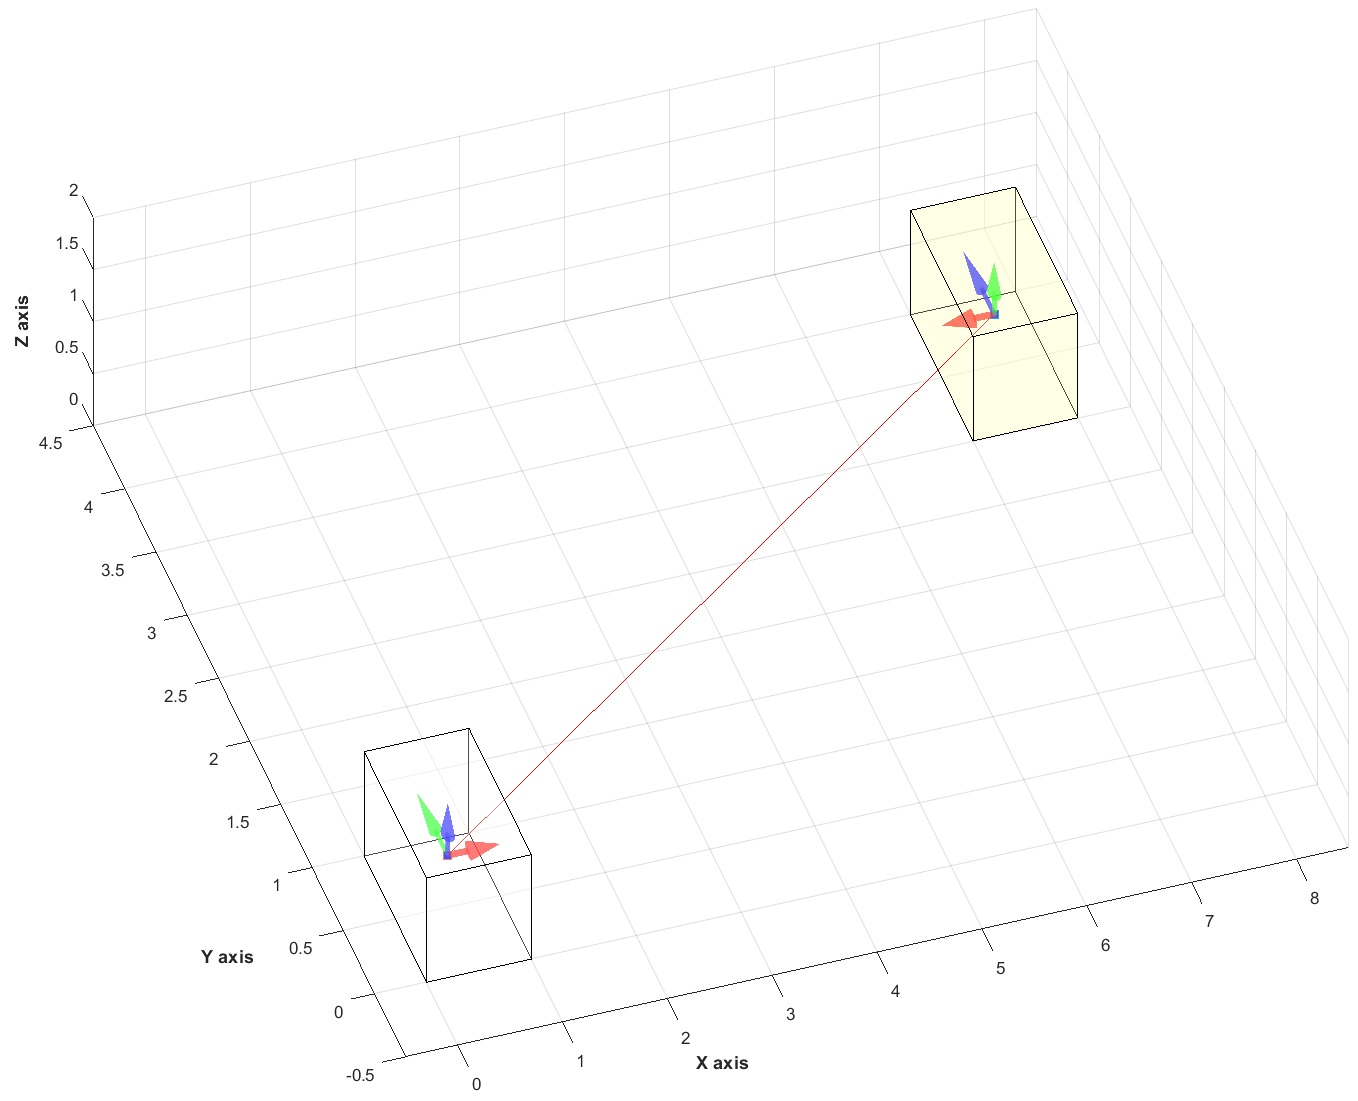
\includegraphics[width=0.5\textwidth]{image/cubePathCase2Initial.jpg}
%			\subcaption{Long distance between two configurations}
%			\label{fig:Cube1Case2}
%		\end{subfigure}
%%\hfill
%		\begin{subfigure}[t]
%			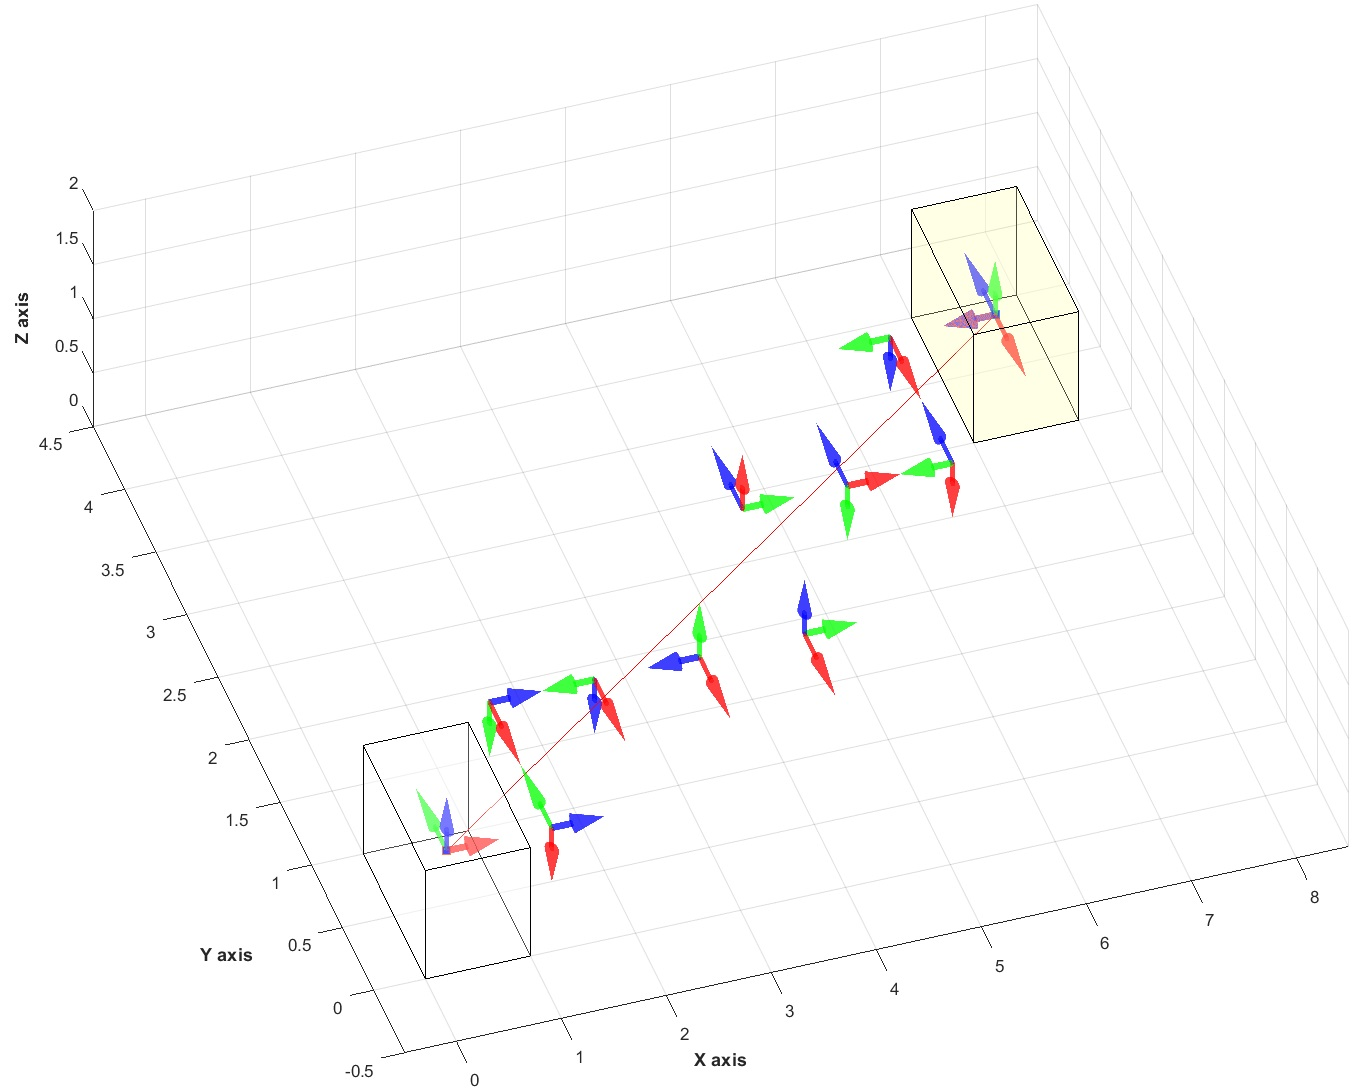
\includegraphics[width=0.5\textwidth]{image/cubePathCase2DirecRolling.jpg}
%			\subcaption{Directly rolling from initial configuration to goal configuration}
%			\label{fig:Cube2Case2}
%		\end{subfigure}
%\end{figure}
\begin{center}
\begin{figure}[h]
\subfigure[Long distance between two configurations]{
	\includegraphics[width=0.5\textwidth]{image/cubeCase2Initial.jpg}
	\label{fig:Cube1Case2}
	}
\hfill
\subfigure[Directly rolling from initial configuration to goal configuration]{
	\includegraphics[width=0.5\textwidth]{image/cubeCase2DirecRolling.jpg}
	\label{fig:Cube2Case2}
	}
\caption{Blah Blah 2}
\end{figure}
\end{center}
%%
%%
%%
\begin{center}
\begin{figure}[h]
\subfigure[Path1]{
	\includegraphics[width=0.5\textwidth]{image/cubeCase2Path1.jpg}
	\label{fig:Cube3Case2}
	}
\hfill
\subfigure[Path2]{
	\includegraphics[width=0.5\textwidth]{image/cubeCase2Path2.jpg}
	\label{fig:Cube4Case2}
	}
\caption{Blah Blah 3}
\end{figure}
\end{center}
%%
%%
%%

\noindent\uline{Case study 3}: Bi-direction path finding.\\
%%
%%
%%

\noindent\uline{Case study 4}: Cube path planning with obstacle avoiding.\\
%%
%%
%%

\noindent\uline{\textbf{Tetrahedron solid}}:
Writing about cube solid properties\\

\noindent\uline{Case study 1}:
Dennis also went his own way and divided the sides of the triangles into equal-angles (as measured from the center of the geodesic), instead of equal-length pieces. This technique is slightly more effective at evenly distributing the triangles across the surface of the sphere. For example, compare an octahedron subdivided with frequency 20, using the linear technique (as outlined by the quiz) versus the angular technique Dennis used in this picture. Note how the linear technique has the triangles piling up along the edges of the original face of the octahedron, where the radial technique does a better job of spacing them out.\\

\begin{center}
\begin{figure}[h]
\subfigure[The initial configuration is the same position but different orientation with goal configuration]{
	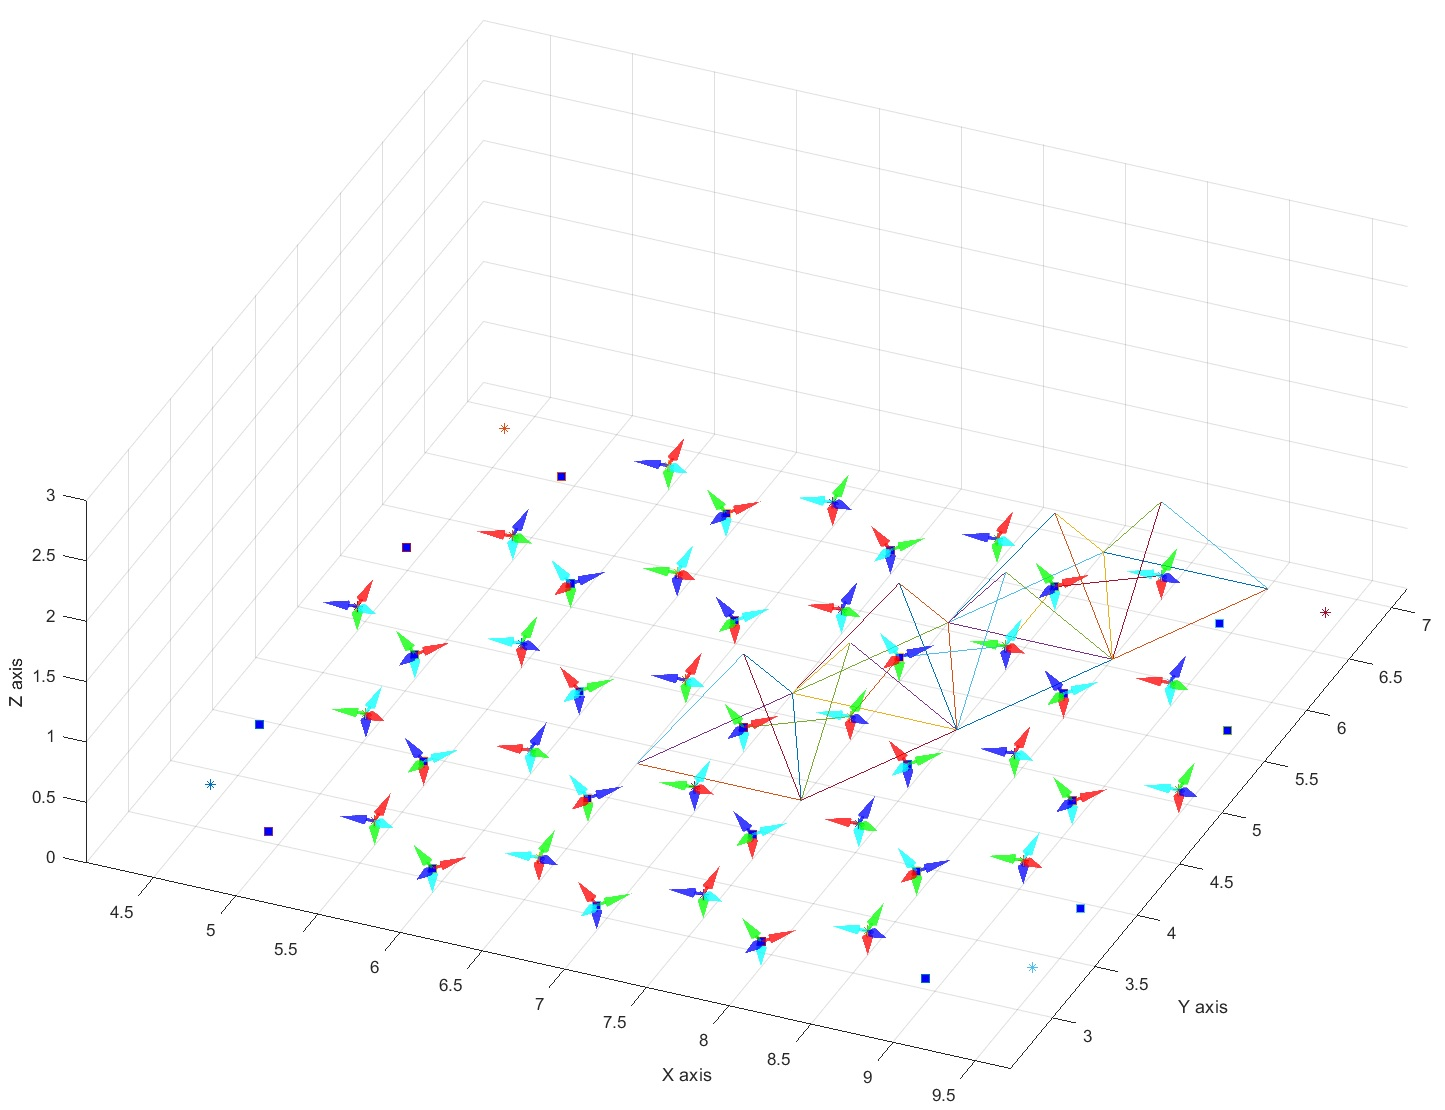
\includegraphics[width=0.5\textwidth]{image/TetraPath1.jpg}
	\label{fig:Tetra1Case1}
	}
\hfill
\subfigure[First four paths of the cube rolling]{
	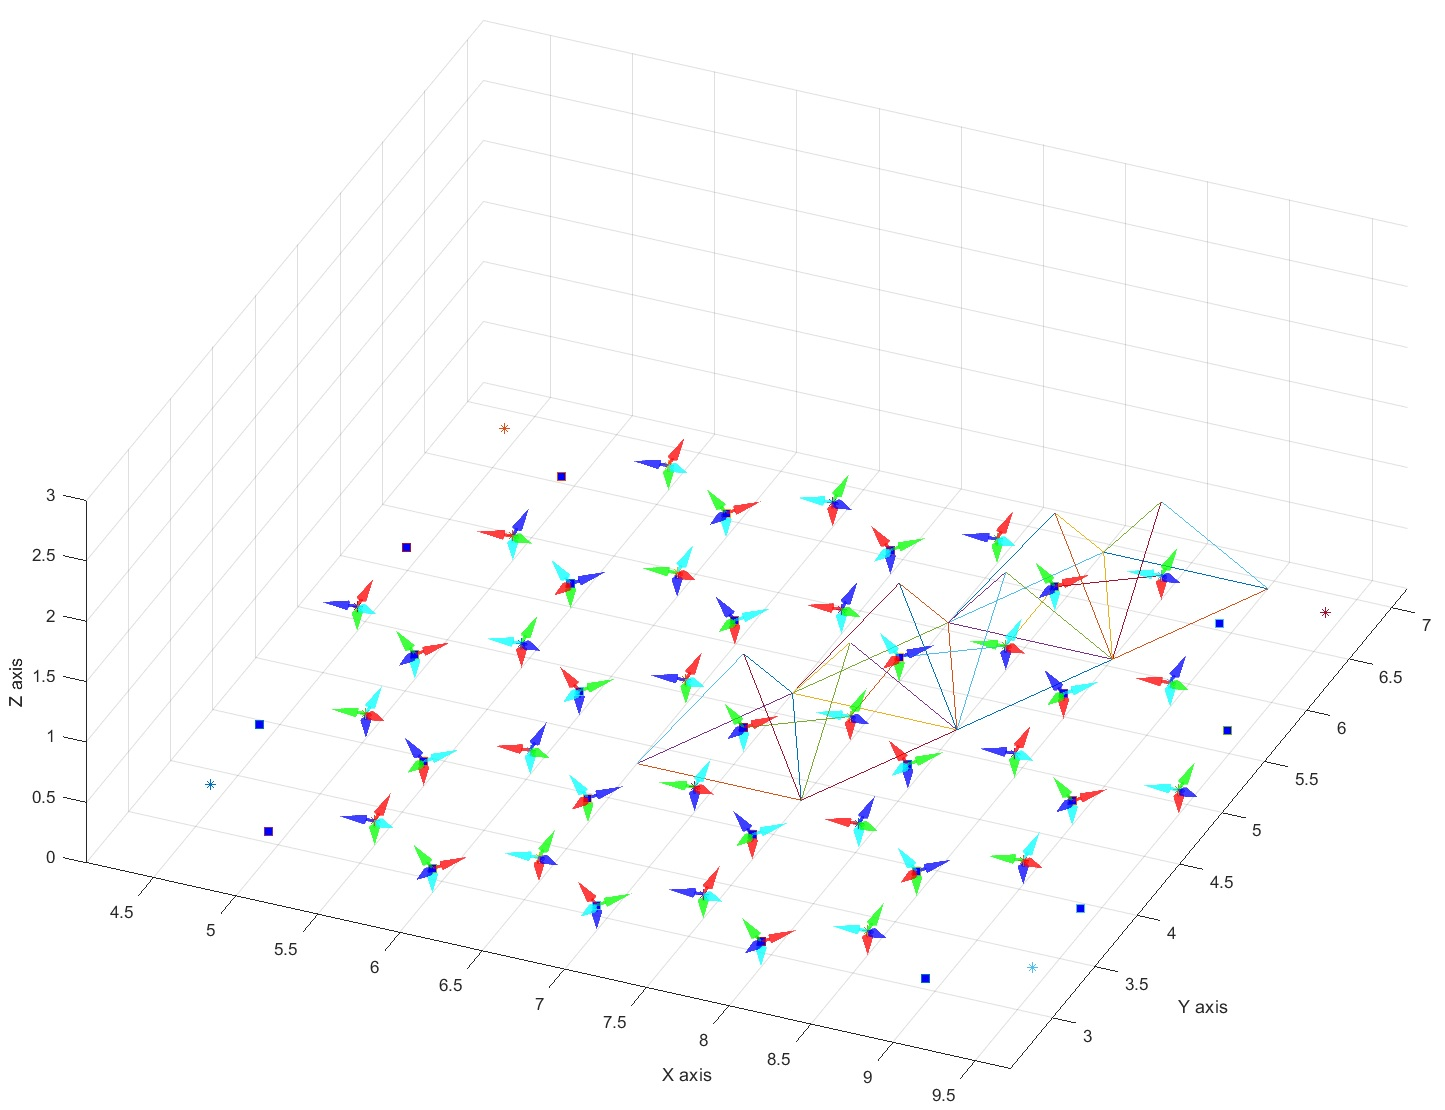
\includegraphics[width=0.5\textwidth]{image/TetraPath1.jpg}
	\label{fig:Tetra2Case1}
	}
\caption{Blah Blah Tetra}
\end{figure}
\end{center}

\noindent\uline{Case study 2}: Long distance between two configuration:
Dennis also went his own way and divided the sides of the triangles into equal-angles (as measured from the center of the geodesic), instead of equal-length pieces. This technique is slightly more effective at evenly distributing the triangles across the surface of the sphere. For example, compare an octahedron subdivided with frequency 20, using the linear technique (as outlined by the quiz) versus the angular technique Dennis used in this picture. Note how the linear technique has the triangles piling up along the edges of the original face of the octahedron, where the radial technique does a better job of spacing them out.\\

\begin{center}
\begin{figure}[h]
\subfigure[The initial configuration is the same position but different orientation with goal configuration]{
	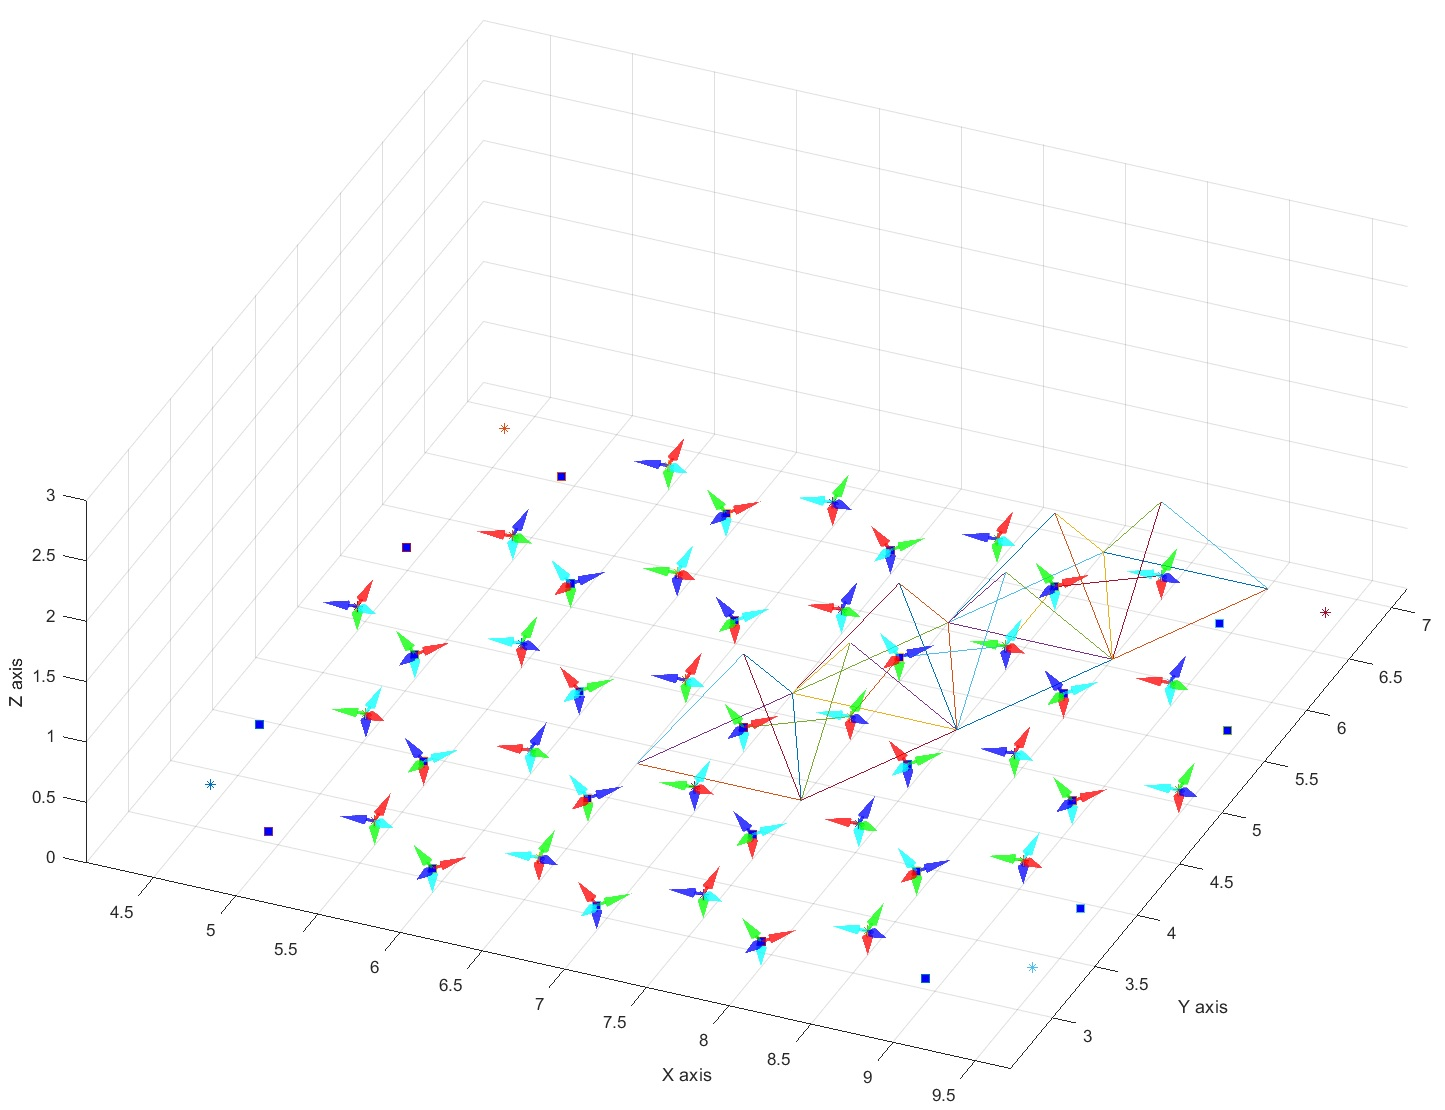
\includegraphics[width=0.5\textwidth]{image/TetraPath1.jpg}
	\label{fig:Tetra1Case1}
	}
\hfill
\subfigure[First four paths of the cube rolling]{
	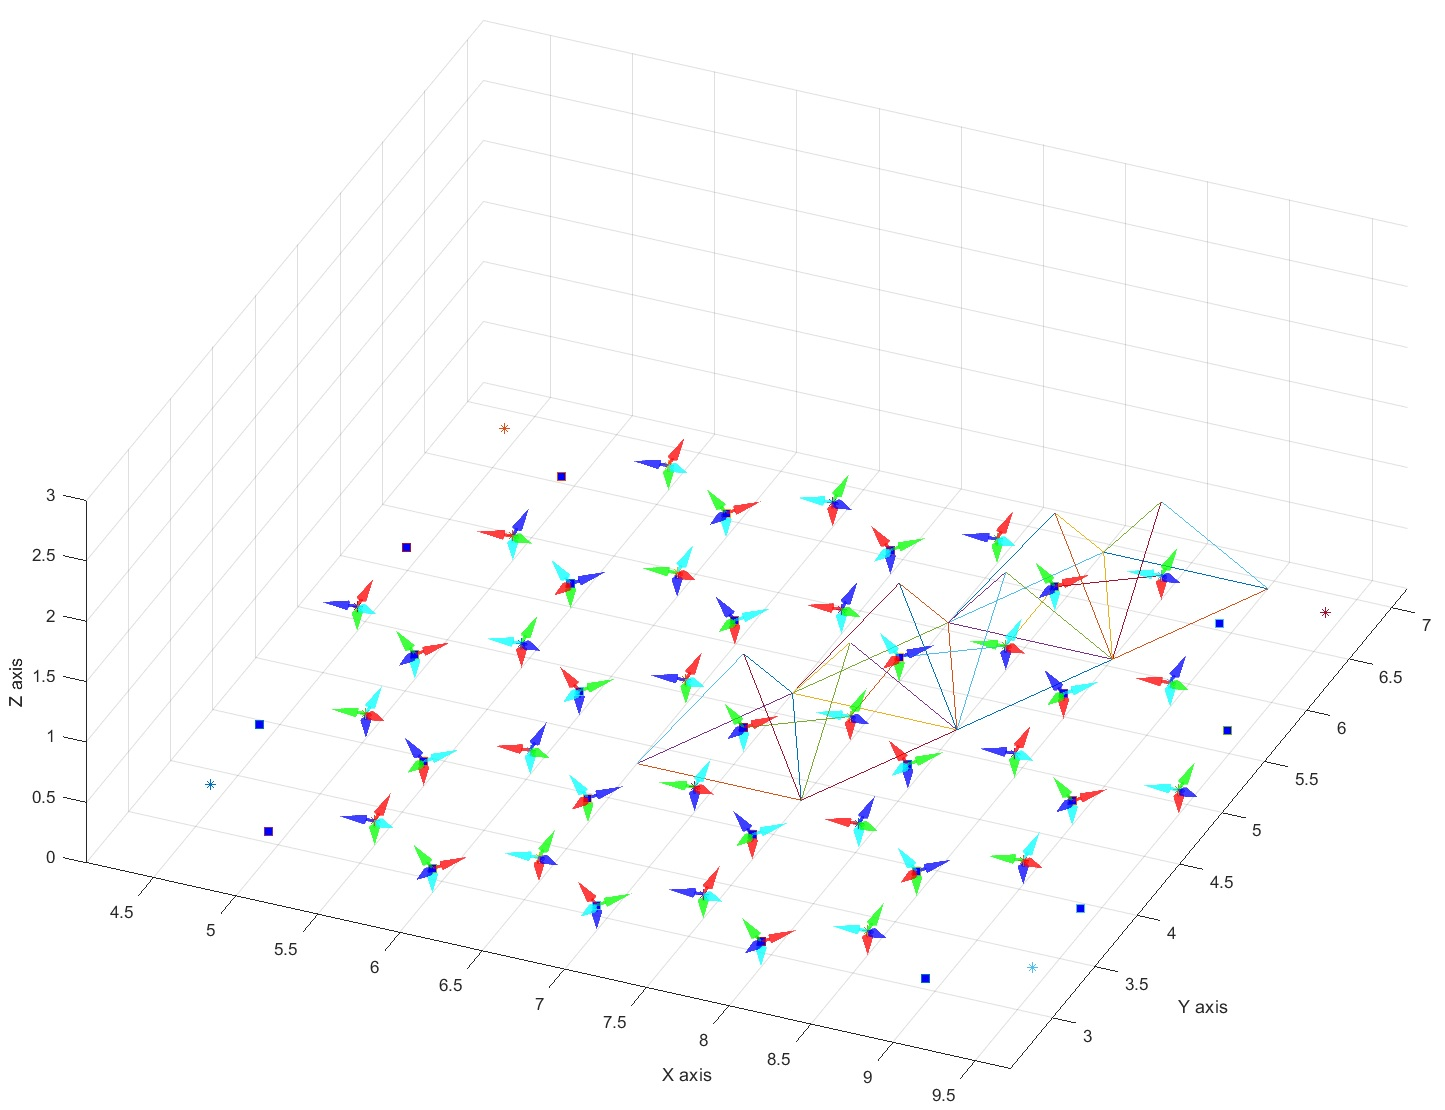
\includegraphics[width=0.5\textwidth]{image/TetraPath1.jpg}
	\label{fig:Tetra2Case1}
	}
\caption{Blah Blah Tetra2}
\end{figure}
\end{center}

%%
%%
%%
%%
\noindent\uline{Case study 3}: Bi-direction path finding.\\
%%
%%
%%

\noindent\uline{Case study 4}: Cube path planning with obstacle avoiding.\\
%%
%%
%%

\noindent\uline{\textbf{Octahedron solid}}:
Writing about cube solid properties\\

\noindent\uline{\textbf{Icosahedron solid}}:
Writing about cube solid properties\\

\noindent\uline{\textbf{Dodecahedron}}:
Writing about cube solid properties\\


\noindent\uline{\textbf{Experiments}}:
Writing about cube solid properties\\

\noindent\uline{\textbf{Discussion}}: Q2 \& Q3\\
- Q2: What are the new things you learned after you did whatever you did?\\
- Q3: What exactly did you do?

\section{CONCLUSION AND FUTURE WORK}
\uline{Questions}: Q4. Why should the community care?\\

\noindent\uline{Should do}: 
- Overview of Q1, Q2, and Q3; plus\\
- What does the community still not know?\\

\noindent\uline{Examples}:
- We have introduced a method of ....\\
- Most of our effort has focused on .... The results of our method often contain .... We believe that there is significant room for improvement by applying ABC methods to the XYZ problem.
- What do we not do?

%%--------------------------
\section{ETHICAL ISSUES}

This research paper will be conducted by the Ph.D. candidate under the guide of supervisors without any ethical issues. No any sensitive data and no harmful chemicals will be used in this research.


\section{DATA STORAGE}

Refer to the Data Management Plan in Appendix \ref{appendix:A}.


\section{FACILITY AND RESOURCES}
Refer to the Table \ref{table:table1}, the facility and resources base on Curtin University and Open Source. \\
\begin{table}[h]
%\setlength{\extrarowheight}{1cm}
	\centering
	\caption{Table of the resources and facilities required for the research and the provider} 
	\begin{tabular}{l l}
	\hline 	
	\bfseries{Resources} &\bfseries{Provider}\\ \hline
	Robot Operating System & Open Source\\
	MatLab                  & Curtin University\\
	BarrettHand             & Curtin University\\
	ABB Robotic Arm         & Curtin University\\
	Computer and Printing   & Curtin University\\
	\hline 
	\end{tabular}
	
	\label{table:table1}
\end{table}




\section{COMPLETION TIMELINES}

\setlength{\arrayrulewidth}{0.1mm}
\setlength{\tabcolsep}{1pt}
\renewcommand{\arraystretch}{1.5}
\newcolumntype{s}{>{\columncolor[HTML]{AAACED}} p{3cm}}


\begin{table}[ht]
\small
\centering
\resizebox{0.8\textwidth}{!}{%
%\resizebox{170mm}{!}{
\begin{tabular}{l*{10}{c}}
\hline
\multicolumn{1}{r}{\textbf{Year}} &\multicolumn{5}{c}{2020} &\multicolumn{5}{c}{2021} \\ \hline
%
\textbf{Activity} & Jan & Mar & May & Aug & Oct & Dec & Jan & Mar & May & Aug \\ \hline
%
Milestone 2 & \cellcolor[HTML]{656565} & \cellcolor[HTML]{656565} & & & & & & & &\\ \hline
%
Optimal Algorithm & &\cellcolor[HTML]{C0C0C0} &\cellcolor[HTML]{C0C0C0} &\cellcolor[HTML]{C0C0C0}  &\cellcolor[HTML]{C0C0C0}  & \cellcolor[HTML]{C0C0C0} & \cellcolor[HTML]{C0C0C0} & \cellcolor[HTML]{C0C0C0} & \cellcolor[HTML]{9B9B9B} & \cellcolor[HTML]{9B9B9B} \\ \hline
%
Simulated approachs & & &\cellcolor[HTML]{C0C0C0}  &\cellcolor[HTML]{C0C0C0}  &\cellcolor[HTML]{C0C0C0}  &\cellcolor[HTML]{C0C0C0}  & \cellcolor[HTML]{C0C0C0} & \cellcolor[HTML]{C0C0C0} & \cellcolor[HTML]{C0C0C0} & \cellcolor[HTML]{9B9B9B} \\ \hline
%
Result \& Validation & & &\cellcolor[HTML]{9B9B9B} &\cellcolor[HTML]{9B9B9B} &\cellcolor[HTML]{9B9B9B} & \cellcolor[HTML]{656565} &\cellcolor[HTML]{9B9B9B} &\cellcolor[HTML]{9B9B9B} &\cellcolor[HTML]{9B9B9B} &  \cellcolor[HTML]{656565}\\ \hline
%
Research papers  &\cellcolor[HTML]{9B9B9B} &\cellcolor[HTML]{9B9B9B} &\cellcolor[HTML]{656565} & \cellcolor[HTML]{9B9B9B} &\cellcolor[HTML]{9B9B9B} & \cellcolor[HTML]{656565} & \cellcolor[HTML]{9B9B9B} & \cellcolor[HTML]{9B9B9B} & \cellcolor[HTML]{656565} & \cellcolor[HTML]{656565}\\ \hline
%
Milestone 3 & & &\cellcolor[HTML]{C0C0C0} &\cellcolor[HTML]{C0C0C0} &\cellcolor[HTML]{C0C0C0} & \cellcolor[HTML]{9B9B9B} & \cellcolor[HTML]{9B9B9B} &\cellcolor[HTML]{9B9B9B} & \cellcolor[HTML]{9B9B9B} & \cellcolor[HTML]{656565}\\ \hline
Thesis preparation & \cellcolor[HTML]{C0C0C0} & \cellcolor[HTML]{C0C0C0} & \cellcolor[HTML]{C0C0C0} & \cellcolor[HTML]{C0C0C0} & \cellcolor[HTML]{9B9B9B} & \cellcolor[HTML]{9B9B9B} & \cellcolor[HTML]{9B9B9B} &  \cellcolor[HTML]{656565} & \cellcolor[HTML]{656565} & \cellcolor[HTML]{656565} \\ \hline
\end{tabular}%
}
\end{table}

\section{DISSEMINATION PLAN}
%The dissemination component of the plan needs to outline how the results of your research will be communicated to your proposed audiences (scholarly, industry, community groups, research participants, broader public). %In this plan you might identify a conference you may present at, and/or the journals you intend to publish in.
\noindent This study solved the problem of closed-path planning for the platonic solids considered for over two decades. The proposed algorithm significantly generates closed-paths faster than RRT* or breath-first search algorithms.
Based on the successful results of the closed-path planning algorithm for rolling polyhedrons on discrete surfaces, this study can be submitted to Science journal in the Report category. 






















%
\newpage
\section{Notes}

Sample file: Links on the class website \url{http://prancer.physics.louisville.edu/classes/308/} \\
Figure \ref{fig:graph1} is an example of  how to do it in \LaTeX \footnote{An example of footnotes}.
\begin{figure}[h]  %t: top, h:exact position
	\begin{center}
	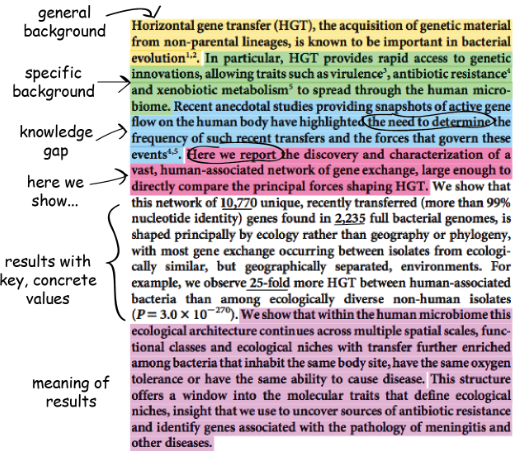
\includegraphics[scale=0.5]{image/good_abstract.png}
	\end{center}
	\caption{The Orion Nebula, M42, recorded with the CDK20N telescope on the night of November 1, 2011.}
	\label{fig:graph1}
\end{figure}

In text $e=mc^2$ and $\frac{1}{2n-1}$.\\

%------------------------------------------
%             tables
%------------------------------------------
\begin{equation}
\frac{x}{y}, \quad
\frac{\delta{f}}{\delta(x)},\quad
\frac{\partial^{2}{f}}{\partial{x}{^2}}
\end{equation}

   
%------------------------------------------
%             Tikz
%------------------------------------------
\begin{center}
%grid-2D-coordinates

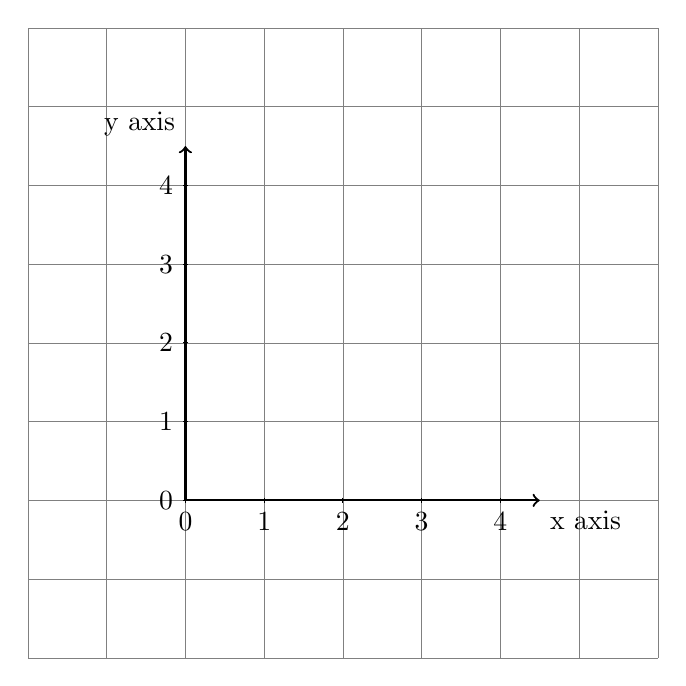
\begin{tikzpicture}
\draw[step=1cm,gray,very thin] (-2,-2) grid (6,6);
\draw[thick,->] (0,0) -- (4.5,0) node[anchor=north west] {x axis};
\draw[thick,->] (0,0) -- (0,4.5) node[anchor=south east] {y axis};

\foreach \x in {0,1,2,3,4}
   \draw (\x cm,1pt) -- (\x cm,-1pt) node[anchor=north] {$\x$};
\foreach \y in {0,1,2,3,4}
    \draw (1pt,\y cm) -- (-1pt,\y cm) node[anchor=east] {$\y$};

\end{tikzpicture}

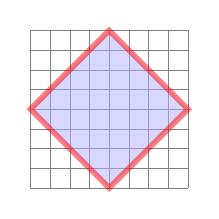
\begin{tikzpicture}
	\draw[step=0.25cm,gray,very thin] (-1,-1) grid (1,1);
	\draw[fill,color=blue!30,draw=red,line width=2pt, opacity=0.5] (1,0) -- (0,1) -- (-1,0) -- (0,-1) -- cycle;
\end{tikzpicture}

\begin{tikzpicture}
	\draw (0,0) grid(5,6);
	\draw (-2,8) rectangle(0,0);
	\draw (0,0) circle (2);
	\draw (5,5) circle (3 and 5);
	\draw (5,8) arc(-90:90:5);
\end{tikzpicture}


\end{center}

%rotation coordinate1
\tdplotsetmaincoords{60}{110}

\begin{tikzpicture}[scale=3,tdplot_main_coords]
\draw[thick,->] (0,0,0) -- (1,0,0) node[anchor=north east]{$x$};
\draw[thick,->] (0,0,0) -- (0,1,0) node[anchor=north west]{$y$};
\draw[thick,->] (0,0,0) -- (0,0,1) node[anchor=south]{$z$};
\coordinate (Shift) at (2,2,2);
\tdplotsetrotatedcoords{-20}{10}{0}
\tdplotsetrotatedcoordsorigin{(Shift)}
\draw[thick,color=blue,tdplot_rotated_coords,->] (0,0,0)
-- (1,0,0) node[anchor=south east]{$x'$};
\draw[thick,color=blue,tdplot_rotated_coords,->] (0,0,0)
-- (0,1,0) node[anchor=west]{$y'$};
\draw[thick,color=blue,tdplot_rotated_coords,->] (0,0,0)
-- (0,0,1) node[anchor=south]{$z'$};
\tdplotsetrotatedthetaplanecoords{30}
\draw[thick,color=blue,tdplot_rotated_coords,->] (0,0,0)
-- (.5,0,0) node[anchor=south east]{$x''$};
\draw[thick,color=blue,tdplot_rotated_coords,->] (0,0,0)
-- (0,.5,0) node[anchor=west]{$y''$};
\draw[thick,color=blue,tdplot_rotated_coords,->] (0,0,0)
-- (0,0,.5) node[anchor=south]{$z''$};
\end{tikzpicture}


%3D_rotation_coordinate
%start tikz picture, and use the tdplot_main_coords style to implement the display 
%coordinate transformation provided by 3dplot


\begin{tikzpicture}[scale=5,tdplot_main_coords]

%Angle Definitions
%-----------------

%set the plot display orientation
%synatax: \tdplotsetdisplay{\theta_d}{\phi_d}
\tdplotsetmaincoords{60}{110}

%define polar coordinates for some vector
%TODO: look into using 3d spherical coordinate system
\pgfmathsetmacro{\rvec}{.8}
\pgfmathsetmacro{\thetavec}{30}
\pgfmathsetmacro{\phivec}{60}
%set up some coordinates 
%-----------------------
\coordinate (O) at (0,0,0);

%determine a coordinate (P) using (r,\theta,\phi) coordinates.  This command
%also determines (Pxy), (Pxz), and (Pyz): the xy-, xz-, and yz-projections
%of the point (P).
%syntax: \tdplotsetcoord{Coordinate name without parentheses}{r}{\theta}{\phi}
\tdplotsetcoord{P}{\rvec}{\thetavec}{\phivec}

%draw figure contents
%--------------------

%draw the main coordinate system axes
\draw[thick,->] (0,0,0) -- (1,0,0) node[anchor=north east]{$x$};
\draw[thick,->] (0,0,0) -- (0,1,0) node[anchor=north west]{$y$};
\draw[thick,->] (0,0,0) -- (0,0,1) node[anchor=south]{$z$};

%draw a vector from origin to point (P) 
\draw[-stealth,color=red] (O) -- (P);

%draw projection on xy plane, and a connecting line
\draw[dashed, color=red] (O) -- (Pxy);
\draw[dashed, color=red] (P) -- (Pxy);

%draw the angle \phi, and label it
%syntax: \tdplotdrawarc[coordinate frame, draw options]{center point}{r}{angle}{label options}{label}
\tdplotdrawarc{(O)}{0.2}{0}{\phivec}{anchor=north}{$\phi$}


%set the rotated coordinate system so the x'-y' plane lies within the
%"theta plane" of the main coordinate system
%syntax: \tdplotsetthetaplanecoords{\phi}
\tdplotsetthetaplanecoords{\phivec}

%draw theta arc and label, using rotated coordinate system
\tdplotdrawarc[tdplot_rotated_coords]{(0,0,0)}{0.5}{0}{\thetavec}{anchor=south west}{$\theta$}

%draw some dashed arcs, demonstrating direct arc drawing
\draw[dashed,tdplot_rotated_coords] (\rvec,0,0) arc (0:90:\rvec);
\draw[dashed] (\rvec,0,0) arc (0:90:\rvec);

%set the rotated coordinate definition within display using a translation
%coordinate and Euler angles in the "z(\alpha)y(\beta)z(\gamma)" euler rotation convention
%syntax: \tdplotsetrotatedcoords{\alpha}{\beta}{\gamma}
\tdplotsetrotatedcoords{\phivec}{\thetavec}{0}

%translate the rotated coordinate system
%syntax: \tdplotsetrotatedcoordsorigin{point}
\tdplotsetrotatedcoordsorigin{(P)}

%use the tdplot_rotated_coords style to work in the rotated, translated coordinate frame
\draw[thick,tdplot_rotated_coords,->] (0,0,0) -- (.5,0,0) node[anchor=north west]{$x'$};
\draw[thick,tdplot_rotated_coords,->] (0,0,0) -- (0,.5,0) node[anchor=west]{$y'$};
\draw[thick,tdplot_rotated_coords,->] (0,0,0) -- (0,0,.5) node[anchor=south]{$z'$};

%WARNING:  coordinates defined by the \coordinate command (eg. (O), (P), etc.)
%cannot be used in rotated coordinate frames.  Use only literal coordinates.  

%draw some vector, and its projection, in the rotated coordinate frame
\draw[-stealth,color=blue,tdplot_rotated_coords] (0,0,0) -- (.2,.2,.2);
\draw[dashed,color=blue,tdplot_rotated_coords] (0,0,0) -- (.2,.2,0);
\draw[dashed,color=blue,tdplot_rotated_coords] (.2,.2,0) -- (.2,.2,.2);

%show its phi arc and label
\tdplotdrawarc[tdplot_rotated_coords,color=blue]{(0,0,0)}{0.2}{0}{45}{anchor=north west,color=black}{$\phi'$}

%change the rotated coordinate frame so that it lies in its theta plane.
%Note that this overwrites the original rotated coordinate frame
%syntax: \tdplotsetrotatedthetaplanecoords{\phi'}
\tdplotsetrotatedthetaplanecoords{45}

%draw theta arc and label
\tdplotdrawarc[tdplot_rotated_coords,color=blue]{(0,0,0)}{0.2}{0}{55}{anchor=south west,color=black}{$\theta'$}

\end{tikzpicture}


\newpage
\begin{center}
\begin{figure}
\subfigure[abc]{
%rotation coordinate1
\tdplotsetmaincoords{60}{110}

\begin{tikzpicture}[scale=3,tdplot_main_coords]
\draw[thick,->] (0,0,0) -- (1,0,0) node[anchor=north east]{$x$};
\draw[thick,->] (0,0,0) -- (0,1,0) node[anchor=north west]{$y$};
\draw[thick,->] (0,0,0) -- (0,0,1) node[anchor=south]{$z$};
\coordinate (Shift) at (2,2,2);
\tdplotsetrotatedcoords{-20}{10}{0}
\tdplotsetrotatedcoordsorigin{(Shift)}
\draw[thick,color=blue,tdplot_rotated_coords,->] (0,0,0)
-- (1,0,0) node[anchor=south east]{$x'$};
\draw[thick,color=blue,tdplot_rotated_coords,->] (0,0,0)
-- (0,1,0) node[anchor=west]{$y'$};
\draw[thick,color=blue,tdplot_rotated_coords,->] (0,0,0)
-- (0,0,1) node[anchor=south]{$z'$};
\tdplotsetrotatedthetaplanecoords{30}
\draw[thick,color=blue,tdplot_rotated_coords,->] (0,0,0)
-- (.5,0,0) node[anchor=south east]{$x''$};
\draw[thick,color=blue,tdplot_rotated_coords,->] (0,0,0)
-- (0,.5,0) node[anchor=west]{$y''$};
\draw[thick,color=blue,tdplot_rotated_coords,->] (0,0,0)
-- (0,0,.5) node[anchor=south]{$z''$};
\end{tikzpicture}


}
\hfill
\subfigure[abc]{
%3D_rotation_coordinate
%start tikz picture, and use the tdplot_main_coords style to implement the display 
%coordinate transformation provided by 3dplot


\begin{tikzpicture}[scale=5,tdplot_main_coords]

%Angle Definitions
%-----------------

%set the plot display orientation
%synatax: \tdplotsetdisplay{\theta_d}{\phi_d}
\tdplotsetmaincoords{60}{110}

%define polar coordinates for some vector
%TODO: look into using 3d spherical coordinate system
\pgfmathsetmacro{\rvec}{.8}
\pgfmathsetmacro{\thetavec}{30}
\pgfmathsetmacro{\phivec}{60}
%set up some coordinates 
%-----------------------
\coordinate (O) at (0,0,0);

%determine a coordinate (P) using (r,\theta,\phi) coordinates.  This command
%also determines (Pxy), (Pxz), and (Pyz): the xy-, xz-, and yz-projections
%of the point (P).
%syntax: \tdplotsetcoord{Coordinate name without parentheses}{r}{\theta}{\phi}
\tdplotsetcoord{P}{\rvec}{\thetavec}{\phivec}

%draw figure contents
%--------------------

%draw the main coordinate system axes
\draw[thick,->] (0,0,0) -- (1,0,0) node[anchor=north east]{$x$};
\draw[thick,->] (0,0,0) -- (0,1,0) node[anchor=north west]{$y$};
\draw[thick,->] (0,0,0) -- (0,0,1) node[anchor=south]{$z$};

%draw a vector from origin to point (P) 
\draw[-stealth,color=red] (O) -- (P);

%draw projection on xy plane, and a connecting line
\draw[dashed, color=red] (O) -- (Pxy);
\draw[dashed, color=red] (P) -- (Pxy);

%draw the angle \phi, and label it
%syntax: \tdplotdrawarc[coordinate frame, draw options]{center point}{r}{angle}{label options}{label}
\tdplotdrawarc{(O)}{0.2}{0}{\phivec}{anchor=north}{$\phi$}


%set the rotated coordinate system so the x'-y' plane lies within the
%"theta plane" of the main coordinate system
%syntax: \tdplotsetthetaplanecoords{\phi}
\tdplotsetthetaplanecoords{\phivec}

%draw theta arc and label, using rotated coordinate system
\tdplotdrawarc[tdplot_rotated_coords]{(0,0,0)}{0.5}{0}{\thetavec}{anchor=south west}{$\theta$}

%draw some dashed arcs, demonstrating direct arc drawing
\draw[dashed,tdplot_rotated_coords] (\rvec,0,0) arc (0:90:\rvec);
\draw[dashed] (\rvec,0,0) arc (0:90:\rvec);

%set the rotated coordinate definition within display using a translation
%coordinate and Euler angles in the "z(\alpha)y(\beta)z(\gamma)" euler rotation convention
%syntax: \tdplotsetrotatedcoords{\alpha}{\beta}{\gamma}
\tdplotsetrotatedcoords{\phivec}{\thetavec}{0}

%translate the rotated coordinate system
%syntax: \tdplotsetrotatedcoordsorigin{point}
\tdplotsetrotatedcoordsorigin{(P)}

%use the tdplot_rotated_coords style to work in the rotated, translated coordinate frame
\draw[thick,tdplot_rotated_coords,->] (0,0,0) -- (.5,0,0) node[anchor=north west]{$x'$};
\draw[thick,tdplot_rotated_coords,->] (0,0,0) -- (0,.5,0) node[anchor=west]{$y'$};
\draw[thick,tdplot_rotated_coords,->] (0,0,0) -- (0,0,.5) node[anchor=south]{$z'$};

%WARNING:  coordinates defined by the \coordinate command (eg. (O), (P), etc.)
%cannot be used in rotated coordinate frames.  Use only literal coordinates.  

%draw some vector, and its projection, in the rotated coordinate frame
\draw[-stealth,color=blue,tdplot_rotated_coords] (0,0,0) -- (.2,.2,.2);
\draw[dashed,color=blue,tdplot_rotated_coords] (0,0,0) -- (.2,.2,0);
\draw[dashed,color=blue,tdplot_rotated_coords] (.2,.2,0) -- (.2,.2,.2);

%show its phi arc and label
\tdplotdrawarc[tdplot_rotated_coords,color=blue]{(0,0,0)}{0.2}{0}{45}{anchor=north west,color=black}{$\phi'$}

%change the rotated coordinate frame so that it lies in its theta plane.
%Note that this overwrites the original rotated coordinate frame
%syntax: \tdplotsetrotatedthetaplanecoords{\phi'}
\tdplotsetrotatedthetaplanecoords{45}

%draw theta arc and label
\tdplotdrawarc[tdplot_rotated_coords,color=blue]{(0,0,0)}{0.2}{0}{55}{anchor=south west,color=black}{$\theta'$}

\end{tikzpicture}

}
\end{figure}
\end{center}

%------------------------------------------
%             Objectives
%------------------------------------------
\subsection*{How to write Objectives}
"Provide a clearly defined statement of the objectives of the research." Sometimes only one objective; sometimes one board AIM, and several objectives.\\
Use active verbs, i.e. propose, create, construct, demonstrate, define, establish, differentiate.
\begin{enumerate}[(i)]
  \item The labels consists of sequential numbers.  
  \begin{itemize}
  	\item The individual entries are indicated with a black dot, a so-called bullet.
  	\item The text in the entries may be of any length.
  \end{itemize}
  \item The numbers starts at 1 with every call to the enumerate environment.
\end{enumerate}
%-------------------------------------------------------
%				Dexterous Motion Planning
%-------------------------------------------------------
\noindent\uline{Dexterous motion planning.} The robot dexterous ma


While Okamura \cite{Okamura_2000_Overview_DM} divided dexterous motion planning into two main categories including the motion planning of the object to acquire a desired configuration and the grasp planning in terms of contact forces optimization.\\

\cite{Trinkle90_Planning_DexManipulation, Trinkle_1991_framework_Planning_DM, Munoz95_Dex.Manipulation_Geo}\\

The article \cite{Bicchi_2000_Hands_Dexterous} focused on three main categories namely manipulative dexterity, grasp robustness, and human operability.
\begin{enumerate}
    \item{Manipulative dexterity: the capability of the hand to manipulate objects so as to relocate them arbitrarily for the purposes of the tasks.}
    \item{Grasp robustness is the capability of keeping hold of manipulated objects in spite of all possible disturbances (unexpected forces, erroneous estimates of the object characteristics, etc.) while maintaining a "gentle” enough grip not to cause any damage.}
	\item{Human operability: the allowance for an easy and friendly interface with the human operator.}
\end{enumerate}
%------------------------------------------
%             Dr. Lei Research Proposal
%------------------------------------------
\newpage
\subsection{Dr. Lei Research Proposal}
\subparagraph{1-Aim}
\textcolor{red}{To develop a discrete rolling contact theory for tactile fingertips.}\\

\noindent\uline{Lack of discrete contact theory for tactile fingertips.} Tactile fingertips have been increasingly used in robot hands in recent years to enhance their dexterity and adaptability. The geometric differential properties of the discretised fingertip surfaces need to be approximated to be used. In this respect, tools such as the \textbf{moving frame} and \textbf{curvatures in discrete differential geometry} provide a consistent and computationally efficient method to approximate these entities. However, \textcolor{red}{\textbf{these tools have not been applied to in-hand manipulation}.}\\


\noindent\uline{Novelty and Impact.} This project will also employ the \emph{tools} developed in \emph{discrete differential geometry} \textbf{to establish \textcolor{red}{a discrete contact theory} of discrete surfaces}, which will be integrated into the proposed pure geometric framework. This project will eradicate the barriers that have hindered the progress of in-hand manipulation and enable robot hands to be used in advanced manufacturing and ultimately to have dexterity and adaptability comparable to the human hand.\\

\subparagraph{2-Background}
\begin{itemize}
\item Rolling contact in human in-hand manipulation
\item Rolling contact in robot hands
\item Vectorial kinematics of multifingered hands
\item Lie group and Lie algebra in kinematics multifingered hands
\item Contact theory via Cantan’s moving frame method
\item Singularity theory for in-hand manipulation
\item \textbf{Discrete contact theory for tactile fingertips}. In recent years, tactile sensors have been added to fingertips of robot hands to emulate human sensing in grasping and manipulation \cite{Lei-Bagnell12_Tactile_Autonomous, HaoDang11_Tactile_BlindGrasping, Rothling07_Dex.Manipulators_Tactile, Zhang14_Tactile_DynamicGrasping}. These grid-based tactile sensors naturally discretise the surfaces of fingertips into \emph{quadrilateral faces}, where the discrete equivalents of notions and methods in differential geometry, such as \textbf{curvatures and the moving frame method}, can be extended \cite{Bobenko10_Discrete_Curvature, Sullivan08_Curvature_DiscreteSurface}. 

Recent progress in discrete differential geometry introduces tools to \textbf{approximate geometric attributes}, especially \textbf{the moving frames and curvatures}, which are guaranteed \emph{to be appropriate extension from the continuous to the discrete setting} \cite{Meyer03_Discrete_Diff.Geo_2Manifolds, Xu13_Geo.Diff_Discrete, Hameiri03_Darboux_Curvature_Discrete}. However, \textcolor{red}{these new tools have not been applied to in-hand manipulation}.
\end{itemize}



\begin{itemize}
\item [25] H. Dang, J. Weisz, and P. K. Allen, "Blind grasping: Stable robotic grasping using tactile feedback and hand kinematics,"
\item [26] F. Röthling."Platform portable anthropomorphic grasping with the bielefeld 20-dof shadow and 9-dof tum hand," 
\item [27] T. Zhang. "Multifingered robot hand dynamic grasping control based on fingertip three-axis tactile sensor feedback," 
\item [28] A. I. Bobenko."A curvature theory for discrete surfaces based on mesh parallelity,"
\item [29] J. M. Sullivan, "Curvatures of smooth and discrete surfaces," in Discrete differential geometry
\item [30] M. Meyer,"Discrete differential-geometry operators for triangulated 2-manifolds," 
\item [31] G. Xu, "Consistent approximations of several geometric differential operators and their convergence,"
\item [32] E. Hameiri. "Estimating the principal curvatures and the Darboux frame from real 3-D range data,"
\end{itemize}

\subparagraph*{3-Significance} \mbox{}\\

\uline{\textcolor{red}{A new discrete rolling contact theory.}} The moving frame method and curvature theory in differential geometry have their counterparts in discrete differential geometry. \textcolor{blue}{An ever increasing number of robot fingertips are equipped with tactile sensors, and these grid-based sensors naturally mesh the fingertips into discrete surfaces} \cite{Lei14_Teleoperation_ThumbRobotHand,  Bagnell12_IntegratedSystem_AutonomousRoboticsManipulation}.
As I pioneered applying \textcolor{blue}{the curvature theory in differential geometry to in-hand manipulation} \cite{Lei09_coordinate-free_instantaneous_kinematics, Lei10_Darboux-Frame, Lei10_Geometric.Kinematics_PointContact, Lei15_PolynomialFormulation_InverseKinematics, Lei15_sliding.rolling.loci_kinematics, Lei09_Kinematic.Geometry_Circular.Surfaces}, I will initiate applying \textcolor{red}{the discrete} \textcolor{blue}{curvature theory} to in-hand manipulation. I will exploit the rich toolset developed in the communities of discrete differential geometry and computer graphics. I will develop a new discrete contact theory
and integrate it into the proposed geometric framework.

\newpage

\cite{Belta_2005_Discrete_MP} (Discrete abstractions for robot motion planning and control in polygonal environments)
\subparagraph{4-Research Design and Method}
\subparagraph*{Overview} Further, I will develop a new discrete contact theory by extending my pioneering work and applying the recent progress in discrete differential geometry.\\

\textbf{Aim 2}: \textbf{To develop a discrete contact theory.}\\

\uline{\textbf{Rationale}}. The grid-based tactile sensors naturally discretise the fingertip surfaces into quadrilateral faces, which can be converted into triangle meshes that have been extensively used in Computer Graphics \cite{Martin04_Quadrilateral_Discrete}. Contact theory requires an approximation of the first and second order properties, such as curvatures and principle directions \cite{Lei10_Darboux-Frame, Montana88_Kinematics_Contact_Grasp}. The current patch-based contact theory needs analytical evaluation, which often introduces overshooting or unexpected surface behaviour. 

On the other hand, moving frame and curvatures can be consistently derived by the rich tool set developed in discrete differential geometry, and these appropriations are guaranteed to be an extension from the continuous to the discrete setting \cite{Meyer03_Discrete_Diff.Geo_2Manifolds}.\\

\uline{\textbf{Theoretical approach}.} I propose to apply \emph{the tool set} developed in \textbf{discrete differential geometry to establish a discrete contact theory}. My contact theory for smooth surfaces is formulated in terms of the moving frame, normal curvature, geodesic curvature, and geodesic torsion [\cite{Lei09_coordinate-free_instantaneous_kinematics, Lei10_Darboux-Frame, Lei15_PolynomialFormulation_InverseKinematics, Lei15_sliding.rolling.loci_kinematics, Lei10_PhDThesis}. \emph{Each of these geometric entities has its counterpart in discrete differential geometry}, as in Fig. 5 (Lei's PhD thesis \cite{Lei10_PhDThesis}). When I was deriving the contact theory, the velocity constraint was embedded in the arc length, \textcolor{red}{eliminating the need of nonlinear differential equations} and \textcolor{blue}{facilitating grid-based path planning}, as in Fig. 6 (in \cite{Lei09_coordinate-free_instantaneous_kinematics}). I \emph{will apply the same approach} in the \emph{discrete case} \textbf{to establish a discrete contact theory} that is coordinate-independent and does not involve difference terms.\\


\uline{\textbf{Empirical validation}.} The BarrettHand is equipped with tactile sensors capable of providing 96 cells of tactile-array data spread across all three fingers and the palm. The density of cells becomes higher towards the very tips of the fingers where finer spatial resolution is desirable \cite{Martin04_Quadrilateral_Discrete}. The embedded signal processing of raw data from the tactile sensors can determine point of contact, and this will facilitate validation of the proposed discrete contact theory.

\subparagraph{Reference}
\begin{itemize}
\item 1 From Dr.LeiCui research : \cite{Lei10_Darboux-Frame, Lei10_Geometric.Kinematics_PointContact, Lei11_Posture.Workspace_Multifinger, Lei12_Polynomial_Inverse.Kinematics, Lei12_ReciprocityBased_SVD_Inverse.Kinematics, Lei15_sliding.rolling.loci_kinematics, Lei15_PolynomialFormulation_InverseKinematics, Lei18_Rolling.Contact_Kinematics_Multifinger, Lei17_In-Hand_Forward.Inverse.Kinematics, Lei07_Euclidean_Invariants, Lei09_Kinematic.Geometry_Circular.Surfaces, Lei09_Orientation-Workspace_Metahand, Lei09_coordinate-free_instantaneous_kinematics}
\item 2 Text book about dynamic-discrete \cite{Book_Rosenberg77_DynamicsDiscrete}
\end{itemize}


%==============================================================
\subsection{Markov Decision Process}
\noindent\uline{Introduction.} 
Markov Decision Process (MDP) is an extension of a Markov chain which is a stochastic model in discrete time. MDP represents a mathematical framework to model decision making process that has been studied in early \cite{Howard60_DP_MDP, Miller68_MDP}. For the record, many applied study may have an implicit underlying the MDP framework to determine the expected cost of raw material that the stock can purchase or shortage \cite{White85_ApplicationMDP}, to control the pest or protect natural resources \cite{White93_ApplicationMDP}. In the robotic field, the MDP has been successfully applied for path planning problems such as combination with a quadtree decomposition of the environment to compute the motion plan \cite{Burlet04_MP_MDP} or association with ideas of deterministic search and dynamic programming techniques to reduce the processing cost and improve performance path planning algorithm \cite{Ferguson04_MDP_Pathplanning}. Another promising technique for autonomous trajectory planning is based on the MDP with clothoid tentacles \cite{Muhager16_MDP_Clothes}. The study used stochastic transitions \cite{Puterman14_Book_MDP_DiscreteDP} that can reduce the presence of distant obstacles in an occupancy grid.\\


%==============================================================
\noindent\uline{The agent-environment interface.} 
As shown in Figure \ref{fig:MDP1}, there are two main objects in the MDP including an agent and the environment that they interact together at each of a sequence of discrete time steps, $t=0,1,2,3,...$. The process in some states $S_t$ at each time step $t$ is described that the decision maker chooses any action $A_t$ in the state and the agent will receive the reward $R_t$ from the environment. In \cite{SuttonBarto18_RLbook}, the general rule of agent-environment boundary is not the same as the physical boundary of a robot's or animal's body. In some cases, the agent may know everything in the environment, just as the rewards which are computed from the agent's action function or the state received. However, in another case of solving puzzle like Rubik's cube, the agent knows all the environment such as colors, faces and dimensions but hard to solve its work.
\begin{figure}[h]
	\begin{center}
	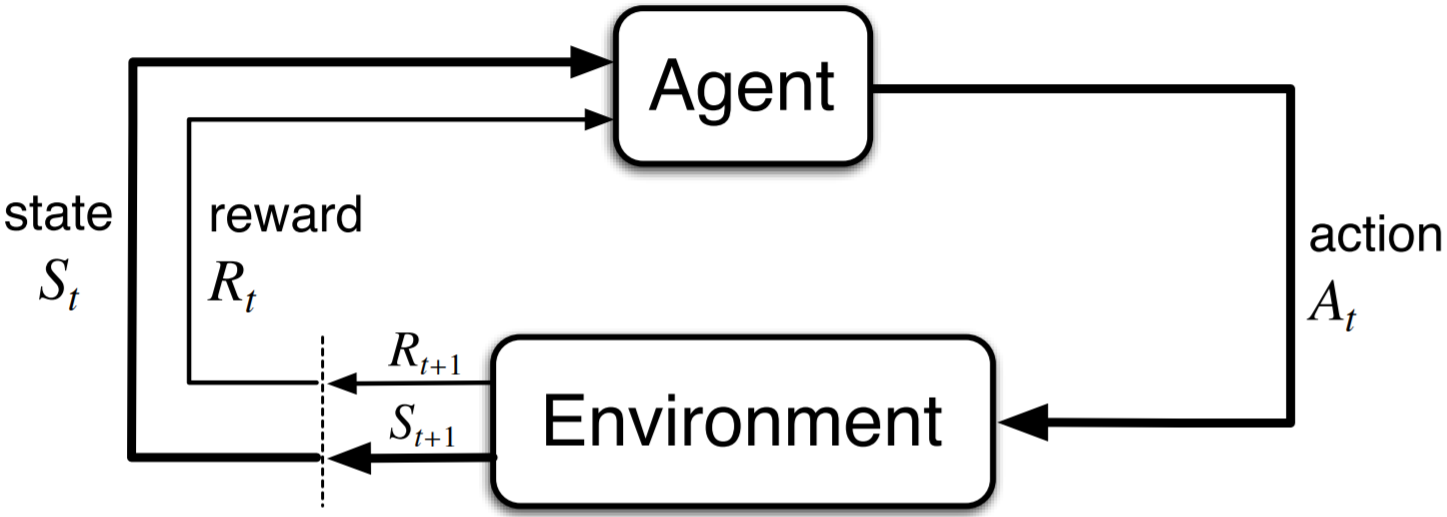
\includegraphics[width=0.5\textwidth]{image/SuttonBartoI_RL.png}
	%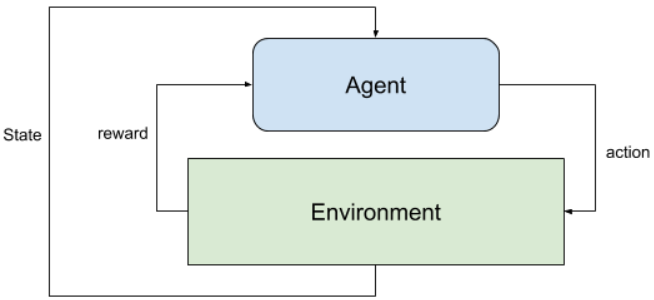
\includegraphics[scale=0.5]{image/MDP.png}
	\end{center}
	\caption{The interaction of agent and environment \cite{SuttonBarto18_RLbook}.}
	\label{fig:MDP1}
\end{figure}


%==============================================================
\noindent MDP is a tuple $<S,A,T,r,\gamma>$ where $S$ is a set of observations when the agent observes a state from the environment; $S$ is a set of actions that the agent can execute from the task to interact with the environment; $T$ is transition probability matrix in which of making the action $a \in A$ from the current state $s \in S$ to the next state $s'$ ($T(s'|s,a)=\mathbb{P}[S_t=s, A_t=a]$); $r$ is the reward model that the agent can receive in the state $s$ when executing an action $a$ ($r(s,a)=\mathbb{E}[R_{t+1}|S_t=s, A_t=a]$), and $\gamma$ is the discount factor where $0<\gamma<1$ that relatives between immediate and future rewards. In path planning problems, the MDP method is applied for finding the path in terms of optimizing the expected sum of discounted rewards and the Bellman equation \cite{Bellman57_MDP} can be promoted in the study.\\ 

%==============================================================
%\noindent\uline{Reinforcement learning.} RL is one part of machine learning which does not require the environment model or the dynamic system as well. \\


%==============================================================
\noindent\uline{Bellman equation.} Before discussing the Bellman equation, there are some of principal components of the Reinforcement Learning framework including Reward and Return, Policies, and Value functions which are briefly introduced as following. \\
\noindent In reinforcement learning, there are two types of value function used to optimize the policy including the state value function $
V^{\pi}(s)=\mathbb{E}_{\pi}[R_t|s_t=s]
$ and the action value function $
Q^{\pi}(s,a)=\mathbb{E}_{\pi}[s_t=s,a_t=a]
$. They are the expected returns generated from the state and action under the policy $\pi$.
The value function changes dependently on the policy for the same environment due to that fact that the value of the state changes dependently and expected rewards will be received. The action value function represents the value of taking an action in some state $s$.\\

\noindent If we call $\mathcal{P}$ is the transition probability from starting state $s$, taking action $a$, then ending up in state $s'$, we have 
$
\mathcal{P}^a_{ss'}=pr(s_{t+1}=s'|s_t=s,a_t=a)
$. 
In addition, $\mathcal{R}^a_{ss'}$ is called the expected reward received from starting state $s$, taking action $a$, and moving into state $s'$, we have 
$
\mathcal{R}^a_{ss'}=\mathbb{E}[r_{t+1}|s_t=s,s_{t+1}=s',a_t=a]
$

\noindent Finally, the Bellman equation \cite{Bellman57_MDP} can be derived for the on-policy state value function with the results is as follows:
\begin{equation}
V^{\pi}(s) = \sum_{a}\pi(s,a)\sum_{s'}\mathcal{P}^a_{ss'}[\mathcal{R}^a_{ss'}+\gamma{V}^{\pi}(s')]
\end{equation}
and for the on-policy action value function as:
\begin{equation}
Q^{\pi}(s,a) = \sum_{s'}\mathcal{P}^a_{ss'}[\mathcal{R}^a_{ss'}+\gamma\sum_{a'}\pi(s',a'){Q}^{\pi}(s',a')]
\end{equation}
for all $s\in{S}, a\in{A(s)}$.

\noindent It is noticed that the Bellman equation can represent the values of states as values of other states like easily calculating the value of state $s_t$ when knowing the value of state $s_{t+1}$. However, to apply for the stochastic shortest path problems by using the Bellman equation, there are techniques such as  value iteration, policy iteration, and linear programming should be taken into consideration to solve the Bellman equation. \\

%==============================================================
\noindent\uline{Value iteration.} This is one of the method to find an optimal policy is to determine the optimal value function. The method in detail to converge to the correct $V^*$ values that can be performed by an iterative algorithm \cite{Bellman57_DynamicProgramming, Bertsekas87_DynamicProgramming}. The Bellman equation for the optimal value function is as follows:
\begin{equation}
Q^{*}(s,a) 
= \mathbb{E}[R_{t+1} + \gamma \max_{a'}Q^{*}(S_{t+1},a')|S_{t}=s, A_{t}=a] 
= \sum_{s',r}p(s',r|s,a)[r+\gamma \max_{a'}Q^{*}(s',a')] 
\end{equation}
The algorithm will stop when the value function changes in a small amount of one update of each state (sweep). The combination of one sweep of policy evaluation and one sweep of policy improvement in the value iteration algorithm can make the convergence faster. It is also noted that the value iteration can be obtained when the step of updating the Bellman optimality equation happens and the updated value has to be required maximum over all actions. \\

%==============================================================
\noindent\uline{Policy iteration.} Policy iteration algorithm can be defined as another way of determining an optimal policy in a finite number iteration. The iteration starts with the value function $V(s)$ of the previous policy $\pi$ in each policy iteration as $\pi_0\xrightarrow{E}v_{\pi_0}\xrightarrow{I}\pi_1\xrightarrow{E}v_{\pi_1}\xrightarrow{I}\pi_2\xrightarrow{E} ... {\pi_*}\xrightarrow{E}v_*$, where $\xrightarrow{E}$ denotes a policy evaluation and $\xrightarrow{I}$ indicates a policy improvement. The Bellman equation for the optimal value function as the policy iteration is:
\begin{equation}
V^{*}(s) 
= \max_{a} \mathbb{E}[R_{t+1} + \gamma V^{*}(S_{t+1})|S_{t}=s, A_{t}=a] = \max_{a} \sum_{s',r}p(s',r|s,a)[r+\gamma V^{*}(s')]
\end{equation}
The policy iteration algorithm may converge only few iterations that will be gained the expected infinite discounted reward by executing the policy \cite{SuttonBarto18_RLbook}: 
\begin{equation}
\pi'(s)=argmax_{a}(R(s,a)+\gamma \sum_{s'\in S} p(s',r|s,a)V^{\pi}(s'))
\end{equation}

%==============================================================
\noindent\uline{Linear programming.} Linear programming methods can be used to solve the Bellman equation and they are better than dynamic programming in some cases as less number of states and a potential method in the curse of dimensionality.
The significant application of the linear programming based path planning algorithm is to derive optimal paths for robotics in various kinds of environment \cite{Chasparis05_PP_LinearProgramming}. The article proposed a linear formulation for resource allocation of the path planning issue. Integrating linear programming to a receding horizon implementation for multi-vehicle path planning is introduced as a model simplification. To describe the feasible path planning, the paper also used stochastic models which can propose the current position and predict the future trajectories. Another implementation of linear programming from \cite{Yang12_PP_LinearProgramming} for the path planning problems has been focus on obstacle avoidance. The most advantage of this improvement is to reduce the computation time cost in the real time computation for the path planning process.
%
\section{Table Notes}


\begin{table}[ht]
\centering
\caption{Thicker horizontal lines above and below the table.}
\begin{tabular}{lcc}
\toprule
&Treatment A&Treatment B\\ 
\hline
%\midrule
John Smith&1&2\\
Jane Doe&--&3\\
Mary Johnson&4&5\\
\bottomrule
\end{tabular}
\end{table}%


Sometimes very long tables must be presented which may also go over pages. \\


\begin{table}[ht!]
     \centering
     \caption{Caption text} 
     \begin{tabular}{|p{5cm}|p{5cm}|}
        \toprule 	
	\bfseries{Resources} &\bfseries{Provider}\\ \hline
	Robot Operating Software & Open Source\\
	MatLab                  & Curtin University\\
	ABB Robotic Arm         & Curtin University\\
	Computer and Printing   & Curtin University\\
	\bottomrule
      \end{tabular}
    \end{table}
    
\begin{table}[h]
 \centering
     \caption{Long table} 
\begin{tabularx}{\textwidth}{X|l}
  \textbf{Symptom} & \textbf{Metric} \\
\hline
Class that & ATFD is more than a few\\
Class that & WMC is high\\
Class that & TCC is low\\
\end{tabularx}
\end{table}


\begin{table}[ht]
\caption{Repetition of custom-defined column type.}
\begin{center}
\begin{tabular}{*{3}{V}}
\hline
aaa&bbb&ccc\\
\hline
aaa&bbb&ccc\\
aaa&bbb&ccc\\
\hline
\end{tabular}
\end{center}
\end{table}


\newpage
\section{Reviews from Prof. Jonathan Paxman for PhD Candidacy Proposal}
• Include a discussion of the motivation and advantages for rolling contact for in-hand manipulation\\
•	Reduce the length of the discussion on modelling the kinematics of rolling motion\\
•	Add a brief review of path planning for two general objects under nonholonomic constraints\\
•	Simply the aims: remove specific techniques and algorithms, and describe the broad aim of the project general terms, and in one or two sentences. Ensure that specific objectives are framed so that the aim can be achieved.\\
•	Include a section which describes how a discretised model will be produced such that the discrete planning algorithms described can be applied. How is this discrete model to be obtained from the continuous-time models discussed?\\
•	If optimal planning is discussed, ensure you are specific about in what sense the solution is optimal. In some cases, optimality is not required, only a satisfactory or satisficing solution in the sense of a cost function being below some bound. In such cases, sampling-based solutions (such as RRT) are appropriate.\\
•	Please also review the writing for grammatical correctness (seek some assistance on this if needed).\\
•	Note Robot Operating System (not Software) in Table 1.\\

%%==============================
%%			%references
%%==============================
\cleardoublepage
\printbibliography

%%=============================={}
%%			%Appendix
%%==============================
\cleardoublepage
\appendix
\section{APPENDIX}
\label{appendix:A}

\centering
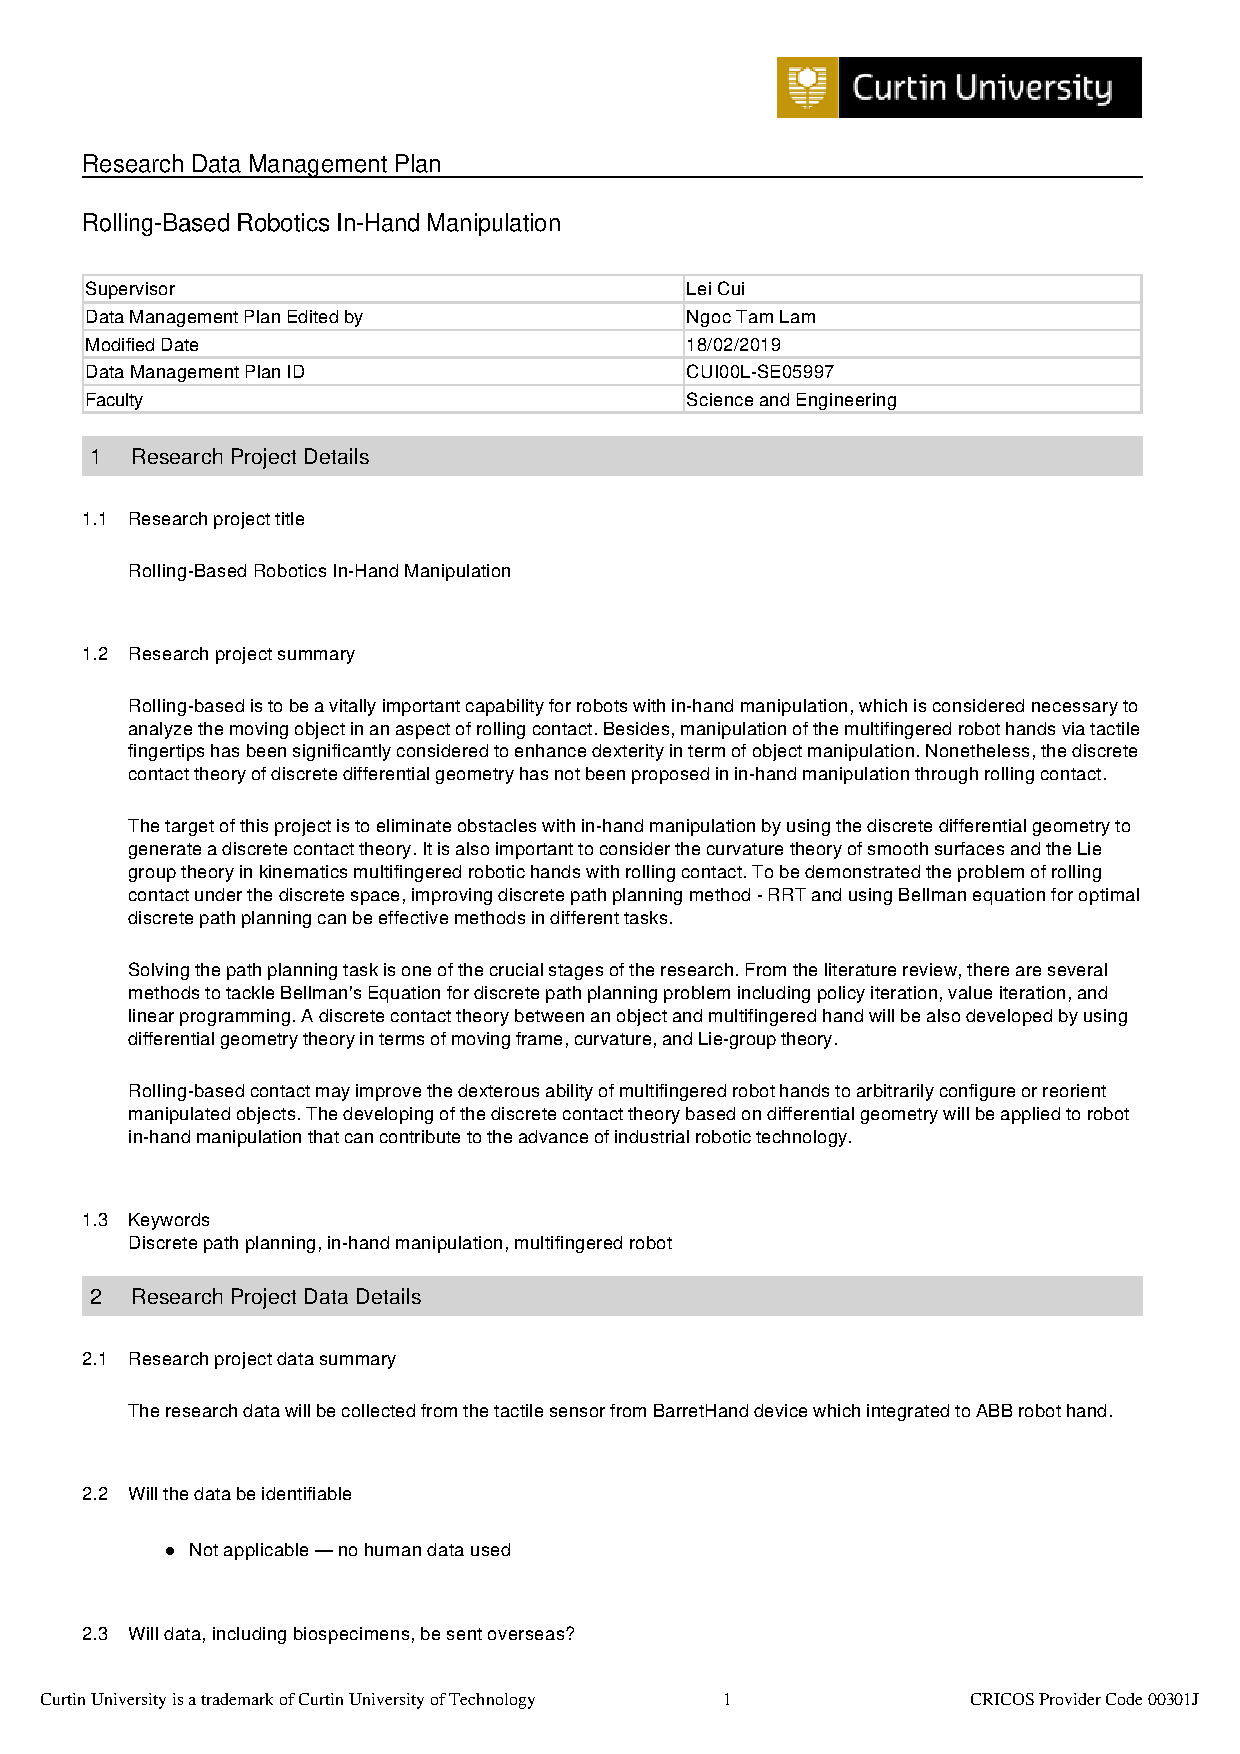
\includegraphics[scale=0.8]{DataManagement.pdf}
\includepdf[pages=2]{DataManagement.pdf}

\end{document}